%----------------------------------------------------------------------------
%----------------------------------------------------------------------------
%%%%%%%%%%%%%%%%%%%%%%%%%%%%%% -*- Mode: Latex -*- %%%%%%%%%%%%%%%%%%%%%%%%%%%%
%% >>slacT486/intro.tex<<
%% Author          : R. Jeffrey Kowalski
%% Created On      : Tue Apr 10 19:50:51 HST 2007
%% Last Modified On: Thu Aug  2 10:54:56 HST 2007
%%%%%%%%%%%%%%%%%%%%%%%%%%%%%%%%%%%%%%%%%%%%%%%%%%%%%%%%%%%%%%%%%%%%%%%%%%%%%%%
From June 19-24, 2006, the experiment, SLAC T486, was performed in the End Station A facility at the Stanford Linear Accelerator Center to measure the Askaryan effect in ice.  28.5 GeV electrons were accelerated with typically 10$^9$ particles in 10 picosecond bunches and delivered into a 7.5 metric tonne target of carving-grade ice to produce electromagnetic showers.  In a dense media like ice, coherent microwave Cherenkov radiation emerges from the particle shower and propagates to the surface of the target where radio antennas can detect the radiation.  This chapter outlines the T486 experiment and the analysis of the Askaryan effect in ice.
%----------------------------------------------------------------------------
%----------------------------------------------------------------------------
\section{Molecular iodine}
The iodine molecule has been extensively studied \cite{Martin:1986a,Wei:1974a,Tellinghuisen:1978a,Gerstenkorn:1981a,Gerstenkorn:1991a,Lamrini:1993a,Lewis:1994a}; we seek to exploit this knowledge base in both our numerical studies and experimental efforts. In the visible region, the absorption spectrum of molecular iodine is dominated by transitions between the ground ``X'' electronic state and an upper excited electronic state called ``B'' \cite{Lewis:1993a}. Here we estimate the required beam parameters for coherent control and introduce the energy level structure.
%----------------------------------------------------------------------------
%----------------------------------------------------------------------------
\subsection{Required (single color) beam properties to control iodine}
%----------------------------------------------------------------------------
\label{iodine}
%----------------------------------------------------------------------------
Suppose the formalism from Section \ref{general dynamics} applies to the molecular iodine system and that there exists a transition in the dominant X-B system \cite{Tellinghuisen:1982a} for which the condition stated in Equation \ref{condition} can be met. The following equation relates $\bar{\mu}_e(R)$ (the electronic contribution to $M$ in the $R$ centroid approximation ) to $M_{ab}$ (from Equation \ref{matrix element}),
%----------------------------------------------------------------------------
\begin{equation}
\boxed{
M_{ab}
=
\bar{\mu}_e(R) \braket
{\nu^{\prime}}
{\nu^{\prime\prime}}
}
\end{equation}
%----------------------------------------------------------------------------
where $\bar{\mu}_e(R)$ is called the electronic transition moment and $\braket{\nu^{\prime}}{\nu^{\prime\prime}}$ is called the Franck--Condon factor (FCF) \cite{Koffend:1979a,Yazykova:1980a,Rapoport:1977a}.

Reference \cite{Lamrini:1993a} reports the squared \emph{electronic} dipole matrix element, $|\bar{\mu}_e(R_c)|^2=|\bar{\mu}_e|^2$, for molecular iodine to vary from a maximum of $(2.00\pm0.11)\mbox{ D}^2$ (or $\bar{\mu}_e \sim 4.7\cross10^{-28}$ Cm) to a minimum of $(8.7\pm4.6)\cross10^{-5}\mbox{ D}^2$ (or $\bar{\mu}_e \sim 5.7\cross10^{-30}$ Cm) for $R_c=2.66\mbox{ \AA}$ and $R_c=6.035\mbox{ \AA}$ respectively ($\mbox{D}=10^{-18}\mbox{ esu}$ and $1\mbox{ Cm}=2.99792458\cross10^{9}\mbox{ esu}$). Reference \cite{Tellinghuisen:1978a} calculates the FCFs for numerous transitions. Most seem to be between $10^{-2}$ and $10^{-3}$; thus, we assume that the transition under consideration here has a FCF in this range. Many transitions have small FCFs, for example for $\nu^{\prime}=\nu^{\prime\prime}=0$ the FCF is $1.429\cross10^{-9}$; however, the density of transitions in molecular iodine is high enough such that we can usually find a strong transition nearby -- even when dealing with a spectral window only a few hundred MHz wide. We will take the logarithmic average of $|M_{+}|=4.7\cross10^{-30}\mbox{ Cm}$ and $|M_{-}|=5.7\cross10^{-33}\mbox{ Cm}$ as an approximate coupling:
%----------------------------------------------------------------------------
\begin{equation}
M
\equiv
|M_{01}|
=
\exp{
\frac{\ln{|M_+|}+\ln{|M_-|}}{2}
}\mbox{ Cm}
\sim
1.6\cross10^{-31}\mbox{ Cm}.
\end{equation}
%----------------------------------------------------------------------------
 In Figure \ref{fluence} we plot Equation \ref{required fluence} (with $\Delta\cdot\tau=\pi/2$) for $M_+$, $M$, and $M_-$.
%----------------------------------------------------------------------------
%----------------------------------------------------------------------------
%----------------------------------------------------------------------------
%bb defines the bounding box for the pdf
%viewport defines the area of the pdf used
%in sidewaysfigure the last entry in bb moves the caption toward/away the pic
%in sidewaysfigure the second entry in bb moves the pic toward/away the caption
%----------------------------------------------------------------------------
\begin{figure}
\scalebox{0.8}[0.8]{
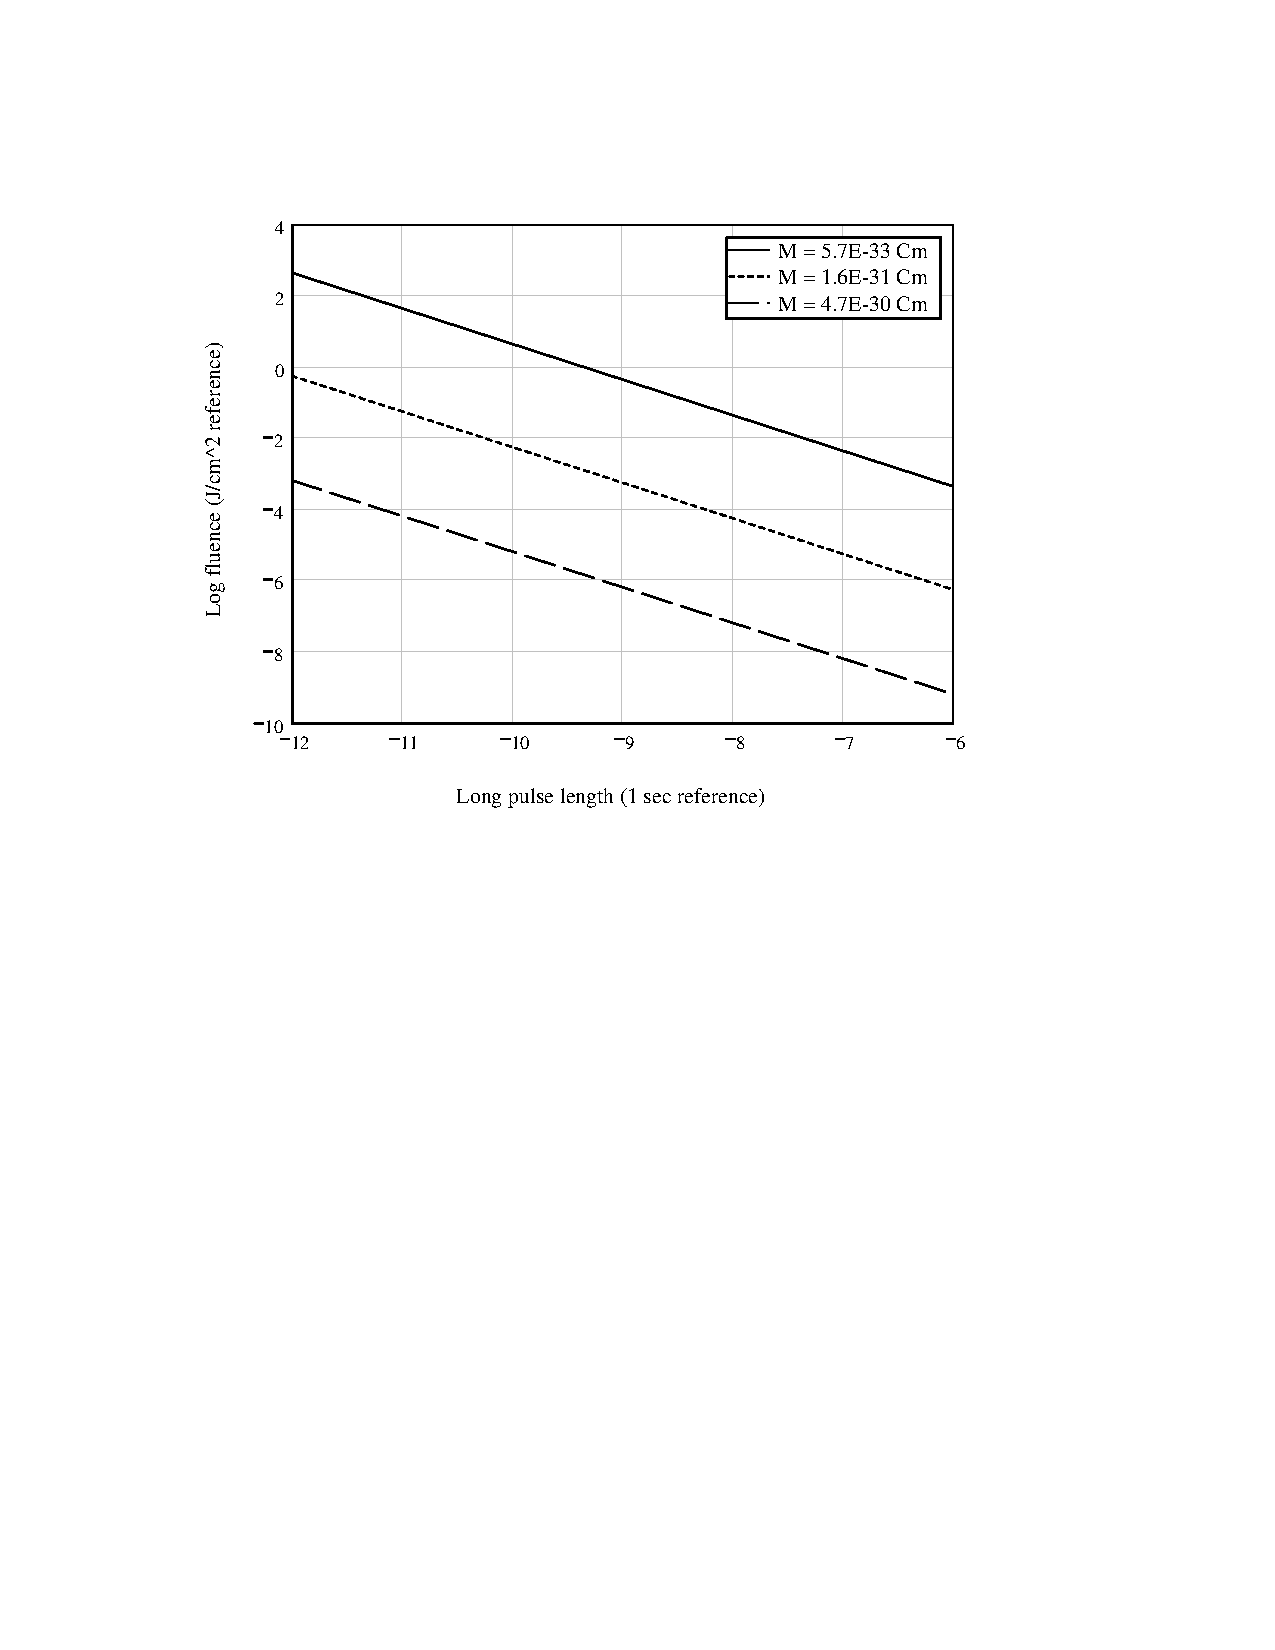
\includegraphics[bb=30 405 489 670]
{fluence/fluence.pdf}
}
\caption[Required fluence for inversion of the two level iodine molecule]{Required fluence for inversion of the two level iodine molecule. Here Equation \ref{required fluence} is plotted for various pulse lengths with $\Delta \tau = \pi/2$. To minimize the effect of collisions on the process, pulse length should be kept less that 1 ns when the target is at atmospheric pressure. A 1 ns pulse focused to a spot with a cross section area of about 1 mm$^2$ will need about 4 mJ to invert the two levels if we assume the ``weak'' coupling ($M=5.7\cross10^{-33}$ Cm). In an evacuated cell, one should be able to reduce the relaxiation effects to allow 100 ns pulses. In this case, the excitation beam (with the same 1 mm$^2$ cross section) must have over 0.7 mW of peak power, even when assuming ``strong'' coupling. ($M=4.7\cross10^{-30}$ Cm)}
\label{fluence}
\end{figure}
%----------------------------------------------------------------------------

%----------------------------------------------------------------------------
%----------------------------------------------------------------------------
%----------------------------------------------------------------------------

%----------------------------------------------------------------------------
\subsection{Energy level model}
%------------------------------------------------------------------------------
\label{iodine levels section}
%------------------------------------------------------------------------------
The two energy levels in consideration here, $X$ and $B$, each consist of many sub levels due to the vibrational and rotational wave functions \cite{Herzberg:1950a}. The dependence of the energy levels on the nuclear spins is small; however, the symmetry properties of the nuclear wave function can still influence the energy transfer during collisions (and influence which molecules couple to the laser field) \cite{Sikora:1997a}. Since we plan to avoid time scales which would allow collisional effects to become significant, we will ignore the nuclear portion of the wave function. When the symmetry rules for dipole transitions between $X$ and $B$ are applied one finds that transitions where $\Delta J=0$ (``Q'' transitions) are forbidden leaving only $\Delta J = \pm 1$ (``P'' and ``R'' transitions).

The vibrational spacing is around 150 cm$^{-1}$ while the rotational spacing corresponding to the P and R transitions ($\Delta J = 2$) is about 10 cm$^{-1}$ for the Boltzmann populated transitions. Since kT is about 200 cm$^{-1}$ at room temperature we see that many rovibrational levels will have significant population within the X electronic state. In fact, there will be hundreds of occupied rovibrational levels in the X band, each connected to tens of rovibrational states (``only'' tens because of the selection rules: the initial and final vibrational states are not constrained; however, the rotational quantum numbers must obey $\Delta J = \pm1$), making thousands of transitions which one would have to track in a model of excitation and fluorescence.

%------------------------------------------------------------------------------
%------------------------------------------------------------------------------
%------------------------------------------------------------------------------
%------------------------------------------------------------------------------
%------------------------------------------------------------------------------

%----------------------------------------------------------------------------
%----------------------------------------------------------------------------
\section{Multi-color LIF simulation}
An estimate of the target/non--target discrimination ratio is calculated in this section. The iodine molecule is selected as the non--target and isotopic iodine 127--129 is used at the target; this is considered a worst case scenario since both molecules will have similar transitions. The key advantage of the three color LIF detection methods presented here is the fact that the fluorescence response of the target can be moved to higher frequencies \emph{without} significant non--target ``following''. The unique blue shifted fluorescence spectrum is found to dominate the non-target's fluorescence in certain spectral windows.
%----------------------------------------------------------------------------
\subsection{The Lorentzian tail}
%----------------------------------------------------------------------------
\label{tail}
%----------------------------------------------------------------------------
The exponentially damped fluorescence response of the excited molecules has a Lorentzian spectral line shape:
%----------------------------------------------------------------------------
\begin{equation}
L(\nu)
=
\frac{1}{\pi}
\frac
{(\Gamma/2)^2}
{(\nu - \nu_{0})^2 + (\Gamma/2)^2}
\label{lorentzian}
\end{equation}
%----------------------------------------------------------------------------
where $\Gamma$ is the FWHM (not related to the density matrix $\Gamma$'s from Section \ref{density formalism}), $\nu_{0}$ is the frequency associated with the fluorescence transition. This is related to the exponential decay by
%----------------------------------------------------------------------------
\begin{equation}
\Gamma=\frac{1}{\pi \tau}
\end{equation}
%----------------------------------------------------------------------------
where $\tau$ is the mean lifetime of the decay. This function is normalized such that
%----------------------------------------------------------------------------
\begin{equation}
\int^{\infty}_{-\infty} L(\nu)d\nu = 1.
\end{equation}
%----------------------------------------------------------------------------

With respect to its peak, the Lorentzian's magnitude decreases by
%----------------------------------------------------------------------------
\begin{equation}
L^{\prime}
=
\frac
{(\Gamma/2)^2}
{(\nu - \nu_{0})^2 + (\Gamma/2)^2}
\sim
\frac{(\Gamma/2)^2}{(\nu - \nu_{0})^2}
\label{norm lorentzian}
\end{equation}
%----------------------------------------------------------------------------
where the latter case holds for $2(\nu - \nu_{0})/\Gamma>>1$. Thus, assuming $\Gamma$ is about twice the FWHM implied by a 1 ns mean lifetime (about 0.02 inverse cm), if we were able to shift the fluorescence energy of the target (i.e. the signal) to a spectral region 1000 cm$^{-1}$ away ($|\nu - \nu_{0}|=1000$ cm$^{-1}$) from the non--traget's fluorescence energy (i.e. noise), the energy of the non--target would be down by 10 orders of magnitude at that spectral location (SNR of 100 dB). For example, if the excitation wavelength is 628 nm (and the non--target emits it's fluroescence energy at this frequency) then this would imply we would need to center our spectrometer at 591 nm or less to ensure the non-target's fluorescence response is reduced by 10 orders of magnitude. This turns out to be an lower bound on the spectral distance since some of the non-target's fluorescence energy will ``follow'' the target's energy to some extent. We approximate the effect of this ``following'' on the SNR in the following sections.
%----------------------------------------------------------------------------
%----------------------------------------------------------------------------
%----------------------------------------------------------------------------
%----------------------------------------------------------------------------
%----------------------------------------------------------------------------
%----------------------------------------------------------------------------
%----------------------------------------------------------------------------
 
%----------------------------------------------------------------------------
\subsection{Dynamics approximation}
%----------------------------------------------------------------------------
\label{approx section}
%----------------------------------------------------------------------------
We seek an approximation to the population dynamics such that we can estimate the final state of a molecular ensemble subject to various pulse sequences (with this information we can build a rough model for the resulting fluorescence spectrum); however, tracking the dynamics (with, for example, Equation \ref{dim eom}) of the thousands of transitions involved would be difficult on a computer. In the following analysis, we ignore the dynamics and assume the probability of level inversion to a function of the detuning only. We also reduce the number of possible pathways to two: the upper electronic state can either populate through a single color transition or a three color ``N'' transition (see Figures \ref{pathways_single} and \ref{pathways_N}). Suppose the probability of some specific transition inverting in a randomly selected molecule, $P$, is given by
%----------------------------------------------------------------------------
%----------------------------------------------------------------------------
%bb defines the bounding box for the pdf
%viewport defines the area of the pdf used
%in sidewaysfigure the last entry in bb moves the caption toward/away the pic
%in sidewaysfigure the second entry in bb moves the pic toward/away the caption
%----------------------------------------------------------------------------
\begin{figure}
\scalebox{0.6}[0.6]{
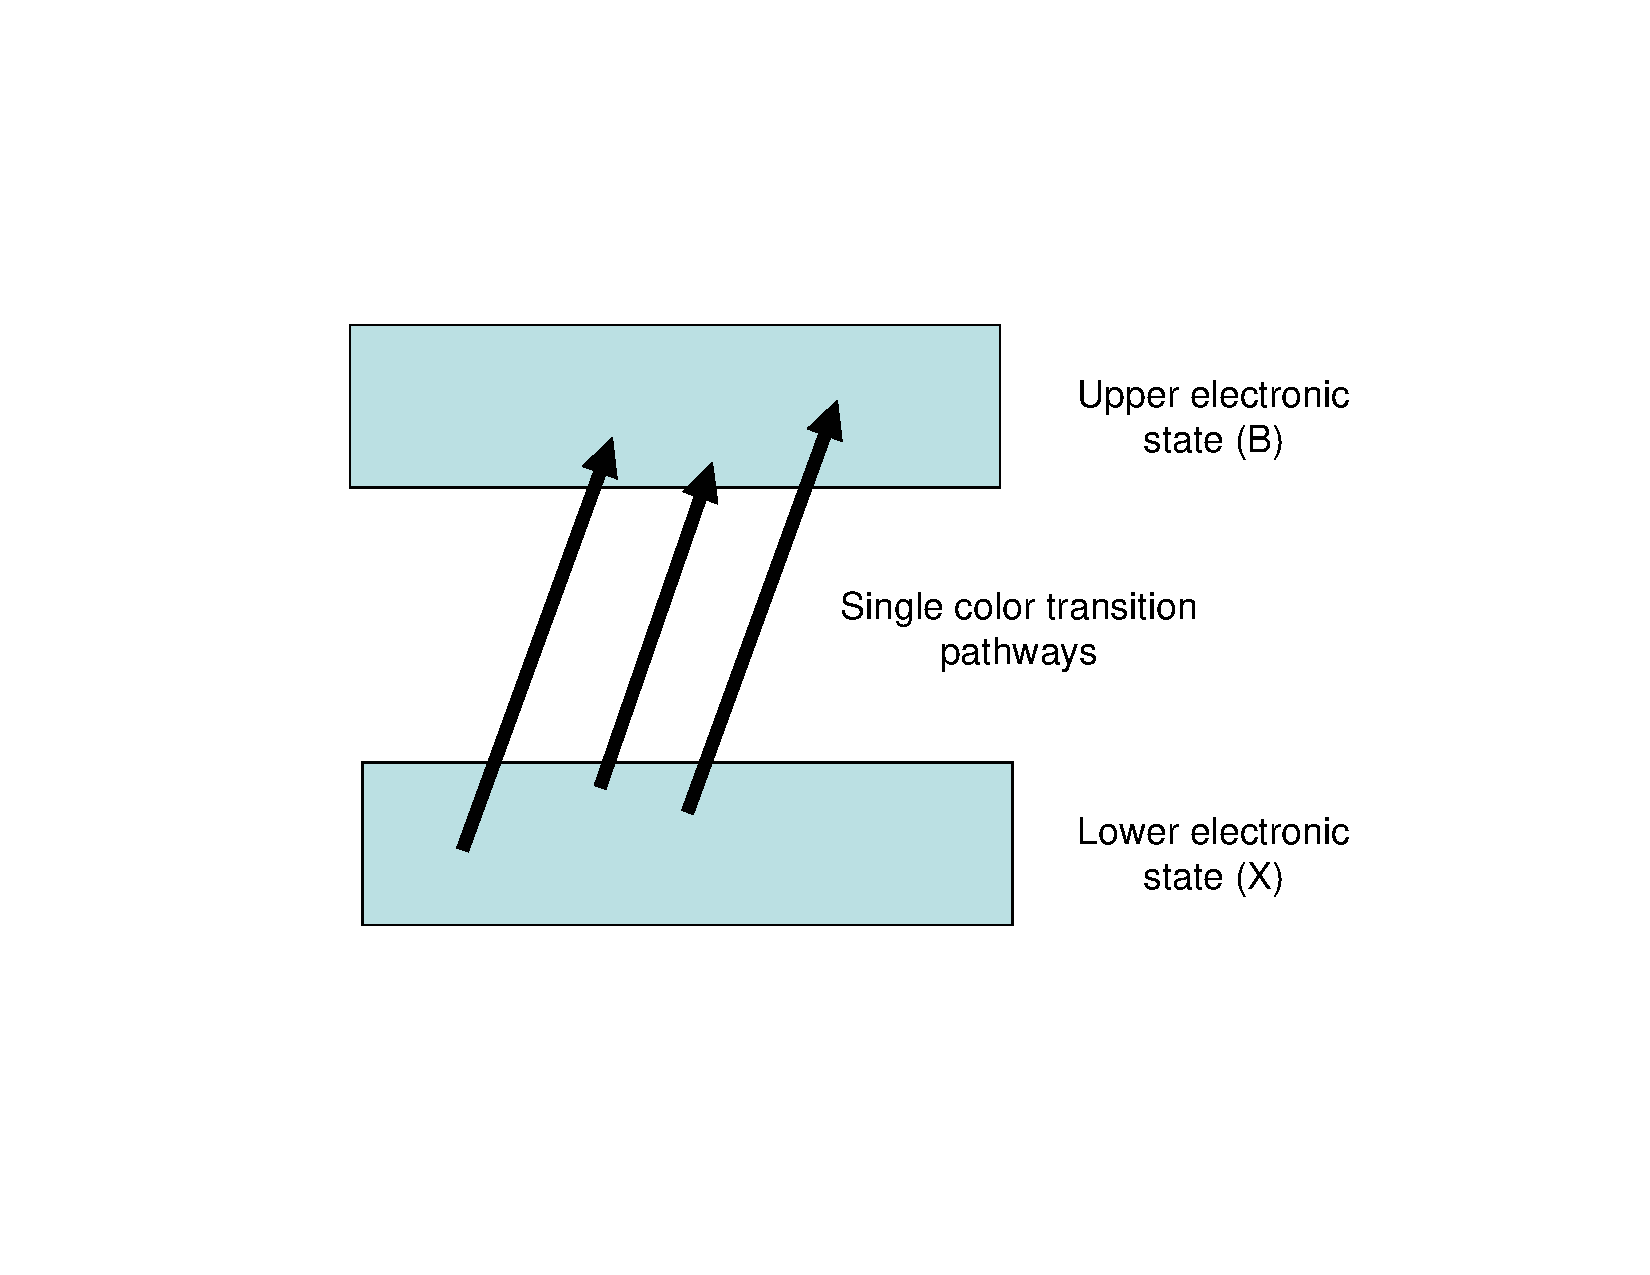
\includegraphics[bb=35 125 489 450]
{pathways_single/pathways_single.pdf}
}
\caption[Single transition diagram]{Single transition diagram. The upper and lower electronic states have a relatively dense substructure of ro-vibrational levels between which we induce transitions.}
\label{pathways_single}
\end{figure}
%----------------------------------------------------------------------------

%----------------------------------------------------------------------------
%----------------------------------------------------------------------------
%----------------------------------------------------------------------------
%bb defines the bounding box for the pdf
%viewport defines the area of the pdf used
%in sidewaysfigure the last entry in bb moves the caption toward/away the pic
%in sidewaysfigure the second entry in bb moves the pic toward/away the caption
%----------------------------------------------------------------------------
\begin{figure}
\scalebox{0.6}[0.6]{
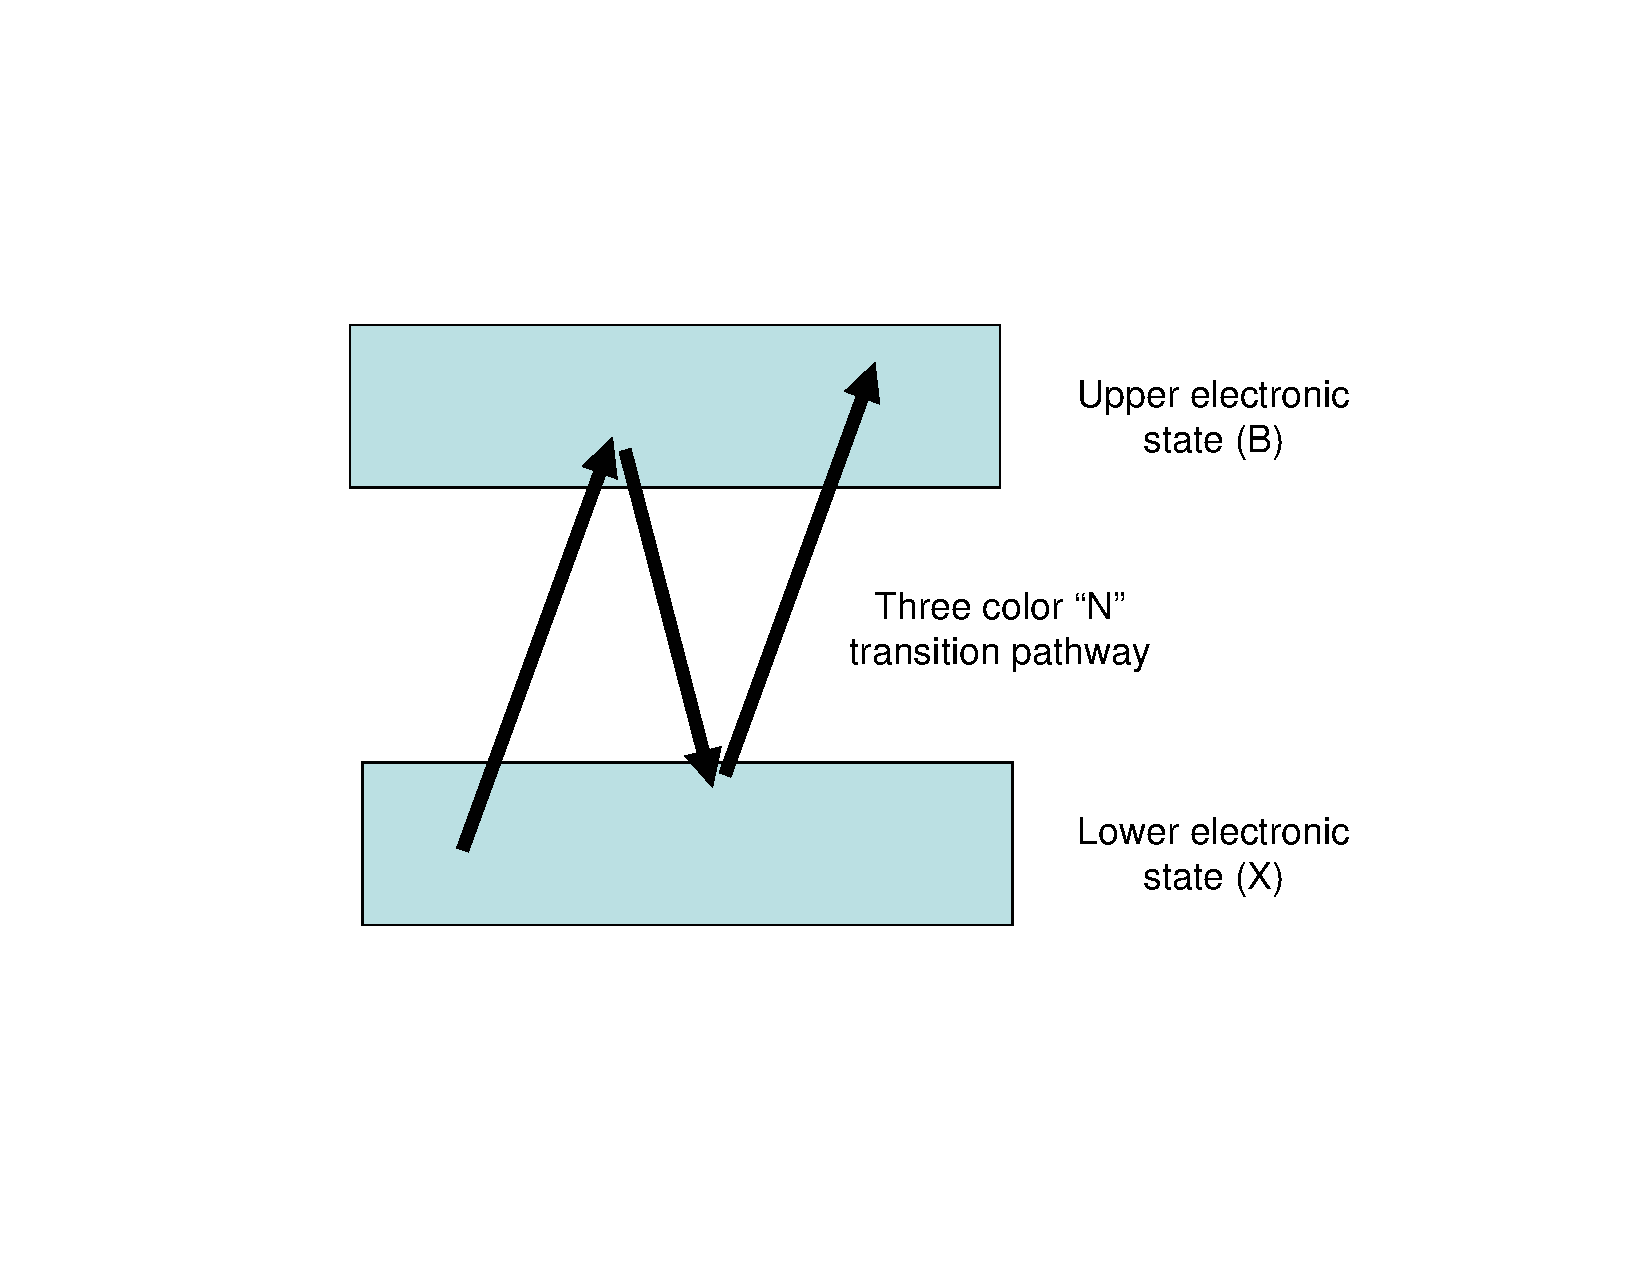
\includegraphics[bb=35 125 489 450]
{pathways_N/pathways_N.pdf}
}
\caption[``N'' transition diagram]{``N'' transition diagram.}
\label{pathways_N}
\end{figure}
%----------------------------------------------------------------------------

%----------------------------------------------------------------------------
%----------------------------------------------------------------------------
\begin{equation}
P(J^{\prime\prime},\nu^{\prime\prime},J^{\prime},\nu^{\prime})
=
L^{\prime}(J^{\prime\prime},\nu^{\prime\prime},J^{\prime},\nu^{\prime})
FCF(\nu^{\prime\prime},\nu^{\prime})
Boltz(\nu^{\prime\prime},\nu^{\prime})
\label{main approx}
\end{equation}
%----------------------------------------------------------------------------
where $L^{\prime}$ is from Equation \ref{norm lorentzian} (in Equation \ref{main approx} $L^{\prime}$ is interpreted as the detuning lineshape for non-resonant excitation; however, in Section \ref{tail} it was used to describe the rate at which fluorescence energy decreases with respect to detuning of the observed spectral window -- same line shape but different process), $FCF$ is the Franck-Condon factor, and $Boltz$ is the normalized Boltzmann probability for population of the lower state (i.e. the probability that the randomly selected molecule occupies the lower state of the transition of interest). In this way we obtain an estimate on the distribution of excited upper states due to single color excitation.

For a three color process (tuned to the target molecule), the second color's effect is treated much the same way except the upper B state becomes the ``source'' for the population transfer. Instead of the $Boltz$ factor we use the $P$'s from the first color; in short, the ensemble of states ``pulled'' up from the X state are ``pushed'' back down to the X state by the second color. Now the third color ``pulls'' this ensemble back up to the B state. In this way we obtain an estimate of the distribution of excited upper states due to three color excitation through a designed resonant pathway (an ``N'' transition).

The goal here is to create a unique population inversion in the target molecule which will glow in the green, while non-targets will glow red. In addition to the resonant pathway described above, there are many pathways one would have to average to gain a good estimate of the actual distribution of the upper states when using an approximation of this type. (The alternative is to track them with Equation \ref{dim eom}.) For the purposes of this argument, we will only compare the resonant pathway to the single color pathway. To support this assumption, the pathway is selected such that the second color pushes the resonant ensemble to an empty region of the X band. In our model we have FCFs for transitions involving lower states with vibrational quantum numbers up to 30: the energy for the X state with $\nu^{\prime\prime}=30$ and $J=0$ is 5916.8561 cm$^{-1}$, more than 29 times kT; so selecting an empty region of the X state is relatively easy.

%----------------------------------------------------------------------------
%----------------------------------------------------------------------------

%----------------------------------------------------------------------------
\subsection{Single vs. three color LIF}
%----------------------------------------------------------------------------
%----------------------------------------------------------------------------
%bb defines the bounding box for the pdf
%viewport defines the area of the pdf used
%in sidewaysfigure the last entry in bb moves the caption toward/away the pic
%in sidewaysfigure the second entry in bb moves the pic toward/away the caption
%----------------------------------------------------------------------------
\begin{figure}
\scalebox{0.8}[0.8]{
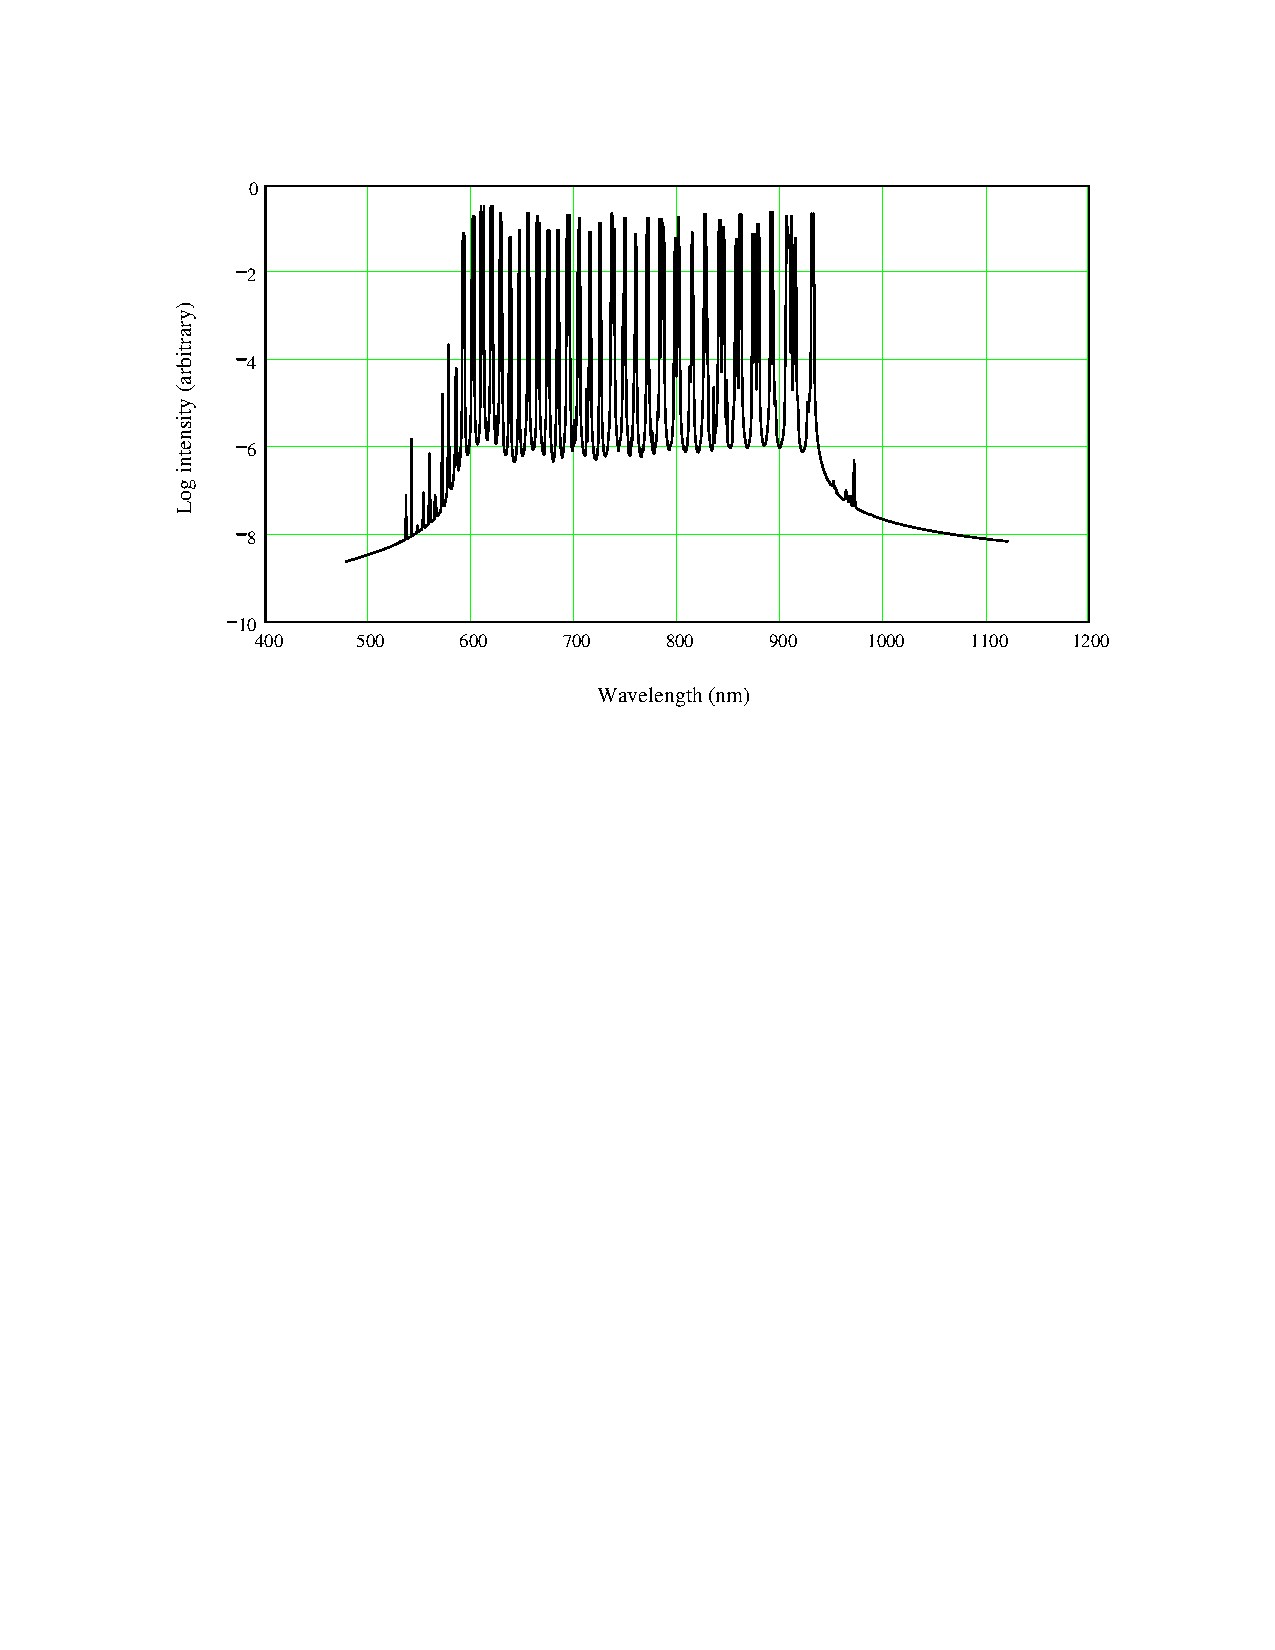
\includegraphics[bb=50 450 489 680]
{non-target_1/non-target_1.pdf}
}
\caption[Simulated single color LIF from non-target molecule (iodine non-isotope)]{Simulated single color LIF from non-target molecule (iodine non-isotope)}
\label{non-target_1}
\end{figure}
%----------------------------------------------------------------------------

%----------------------------------------------------------------------------
%----------------------------------------------------------------------------
From these final upper state distributions a fluorescence spectrum is calculated. Each energy level in the calculated upper B state distribution is connected, in a $J=\pm1$ pair, to each X vibrational state. A ``fluorescence line strength'', $S$, is assigned to each possible downward transition and approximated by
%----------------------------------------------------------------------------
\begin{equation}
S(\nu^{\prime\prime},\nu^{\prime})
=
P^{\prime}FCF(\nu^{\prime\prime},\nu^{\prime})
\end{equation}
%----------------------------------------------------------------------------
%----------------------------------------------------------------------------
%----------------------------------------------------------------------------
%bb defines the bounding box for the pdf
%viewport defines the area of the pdf used
%in sidewaysfigure the last entry in bb moves the caption toward/away the pic
%in sidewaysfigure the second entry in bb moves the pic toward/away the caption
%----------------------------------------------------------------------------
\begin{figure}
\scalebox{0.8}[0.8]{
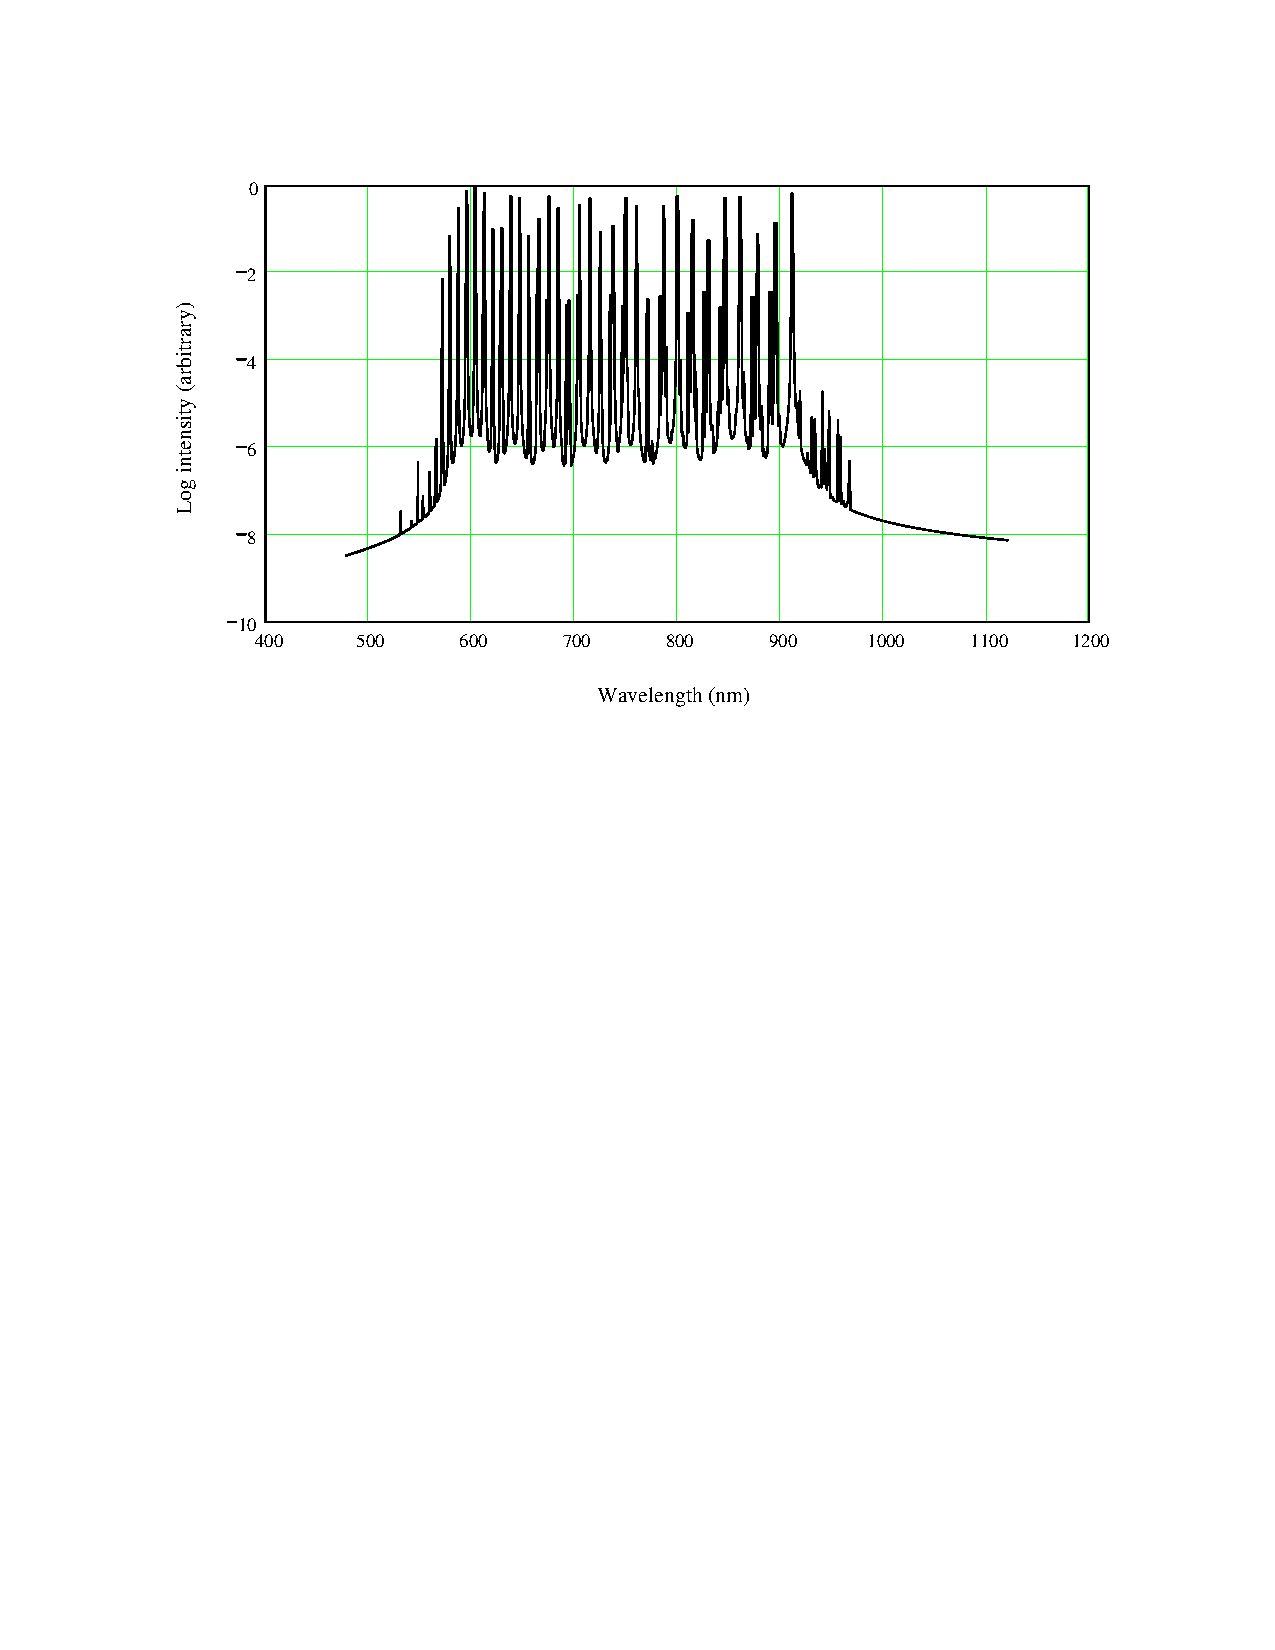
\includegraphics[bb=50 450 489 680]
{target_1/target_1.pdf}
}
\caption[Simulated single color LIF from target molecule (iodine isotope)]{Simulated single color LIF from target molecule (iodine isotope)}
\label{target_1}
\end{figure}
%----------------------------------------------------------------------------

%----------------------------------------------------------------------------
where $P^{\prime}$ is the initial population of the fluoresceing B level ($\nu^{\prime\prime}$) calculated for each pathway, and $\nu^{\prime}$ is the vibrational number of the lower X vibrational level. The resulting fluorescence signal from each transition is modeled by Equation \ref{lorentzian} by assigning each J-split pair to a Lorentzian scaled by $S$. See Figure \ref{non-target_1}, \ref{target_1}, and \ref{target_3} for a plots of the resulting signal from summing the transitions for a few basic pathways. Note that when one considers the result from Section \ref{side} (only around one thousand of iodine molecules emit into the detector in the benchtop geometry) we see that verification of these high extinction ratios becomes unlikely unless we move to a LIDAR type geometry.
%----------------------------------------------------------------------------
%----------------------------------------------------------------------------
%bb defines the bounding box for the pdf
%viewport defines the area of the pdf used
%in sidewaysfigure the last entry in bb moves the caption toward/away the pic
%in sidewaysfigure the second entry in bb moves the pic toward/away the caption
%----------------------------------------------------------------------------
\begin{figure}
\scalebox{0.8}[0.8]{
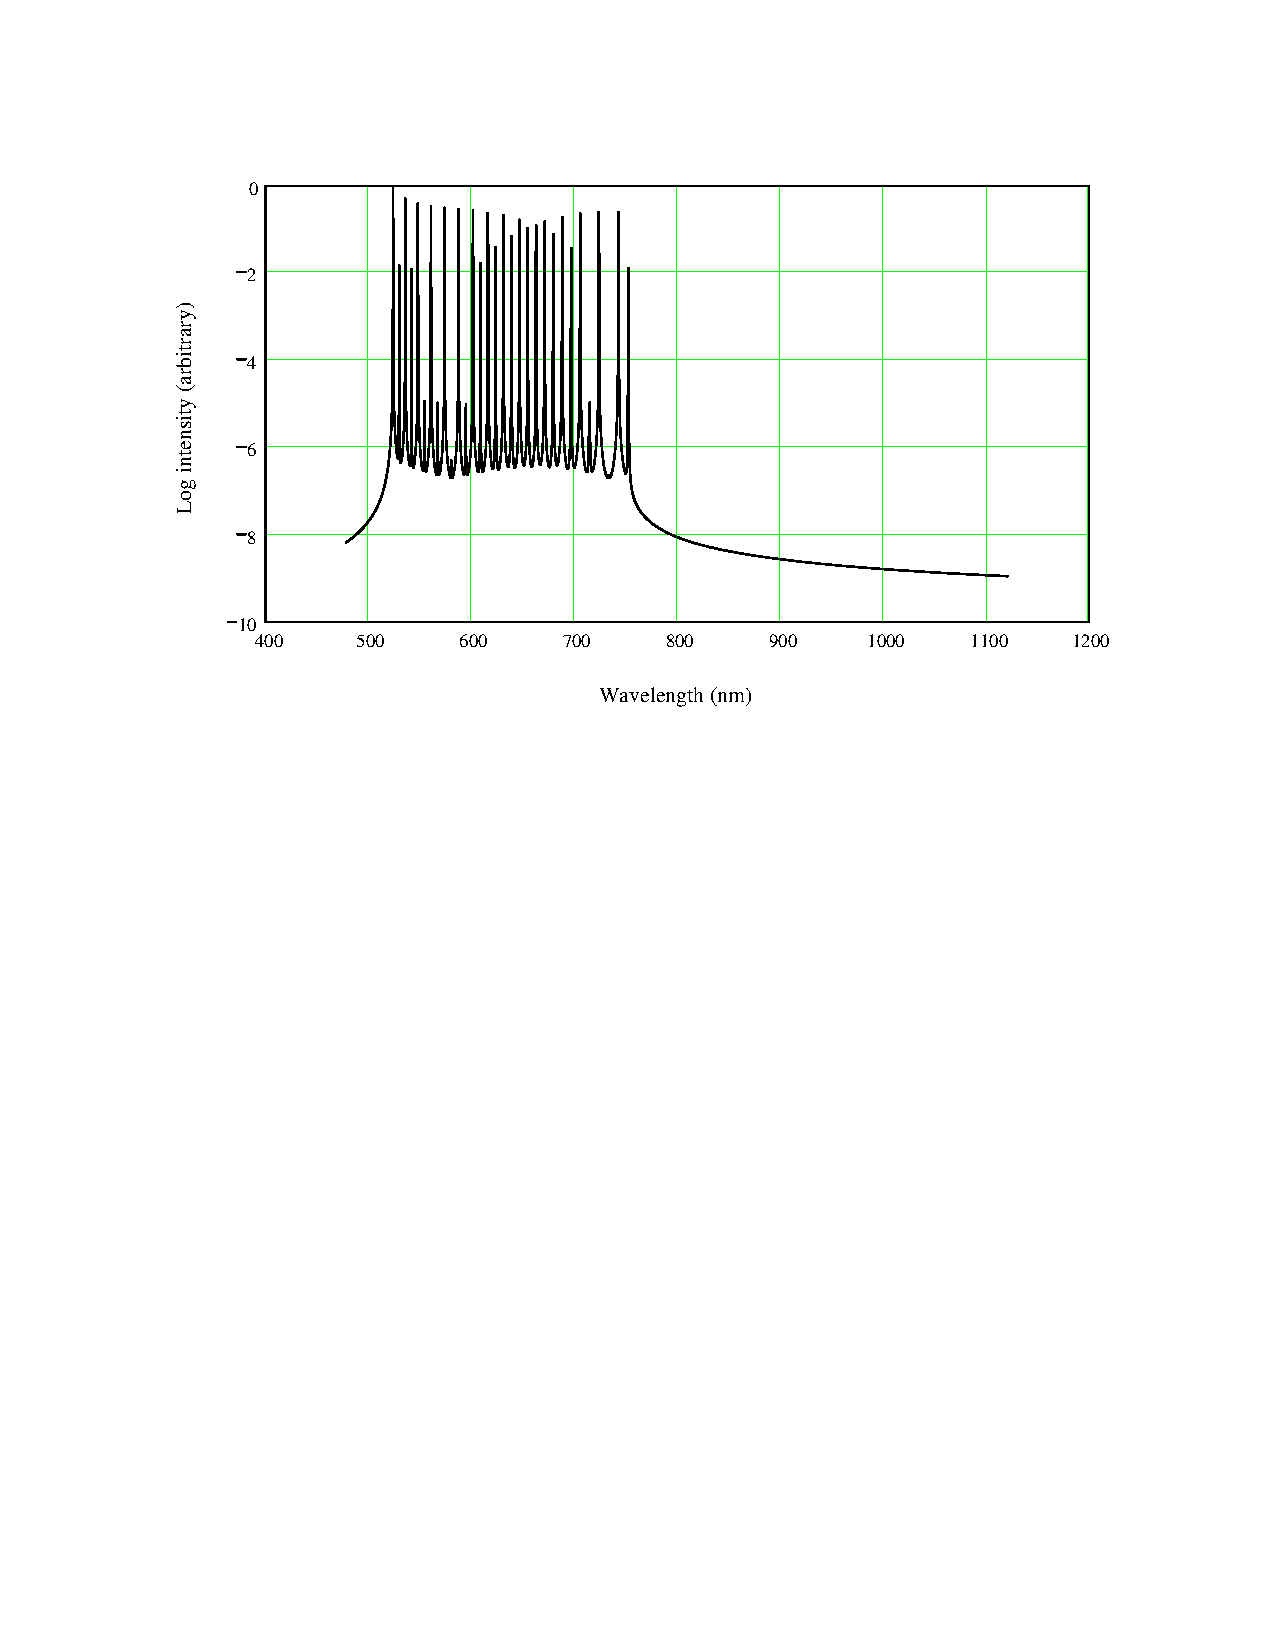
\includegraphics[bb=50 450 489 680]
{target_3/target_3.pdf}
}
\caption[Simulated three color LIF from target molecule (iodine isotope)]{Simulated three color LIF from target molecule (iodine isotope). These simulations show that the three color LIF (shown here) is around 8 orders of magnitude more intense than the single color responce of the target and non-target (see Figures \ref{target_1} and \ref{non-target_1}) in the spectral region near 520 nm.}
\label{target_3}
\end{figure}
%----------------------------------------------------------------------------

%----------------------------------------------------------------------------
%----------------------------------------------------------------------------
%----------------------------------------------------------------------------
%----------------------------------------------------------------------------
%----------------------------------------------------------------------------
%----------------------------------------------------------------------------
%----------------------------------------------------------------------------

%----------------------------------------------------------------------------
%----------------------------------------------------------------------------
\section{Coherent population transfer}
In this section we describe the unique advantages to the coherent control process under investigation. Evidence for an increase in potential LIDAR sensitivity is revealed when one considers the robust population inversion properties of these coherent process. The detuning properties are shown to not have an adverse affect on discrimination and allow near--unity population transfer efficiencies even with non-uniform spatial intensity distributions and shot-to-shot pulse height variations (we re-visit and re-analyze some of the results from Section \ref{random sims}).
%----------------------------------------------------------------------------
\subsection{STIRAP pulse height insensitivity}
%----------------------------------------------------------------------------
%----------------------------------------------------------------------------
%----------------------------------------------------------------------------
%----------------------------------------------------------------------------
%bb defines the bounding box for the pdf
%viewport defines the area of the pdf used
%in sidewaysfigure the last entry in bb moves the caption toward/away the pic
%in sidewaysfigure the second entry in bb moves the pic toward/away the caption
%----------------------------------------------------------------------------
\begin{figure}
\scalebox{1}[1]{
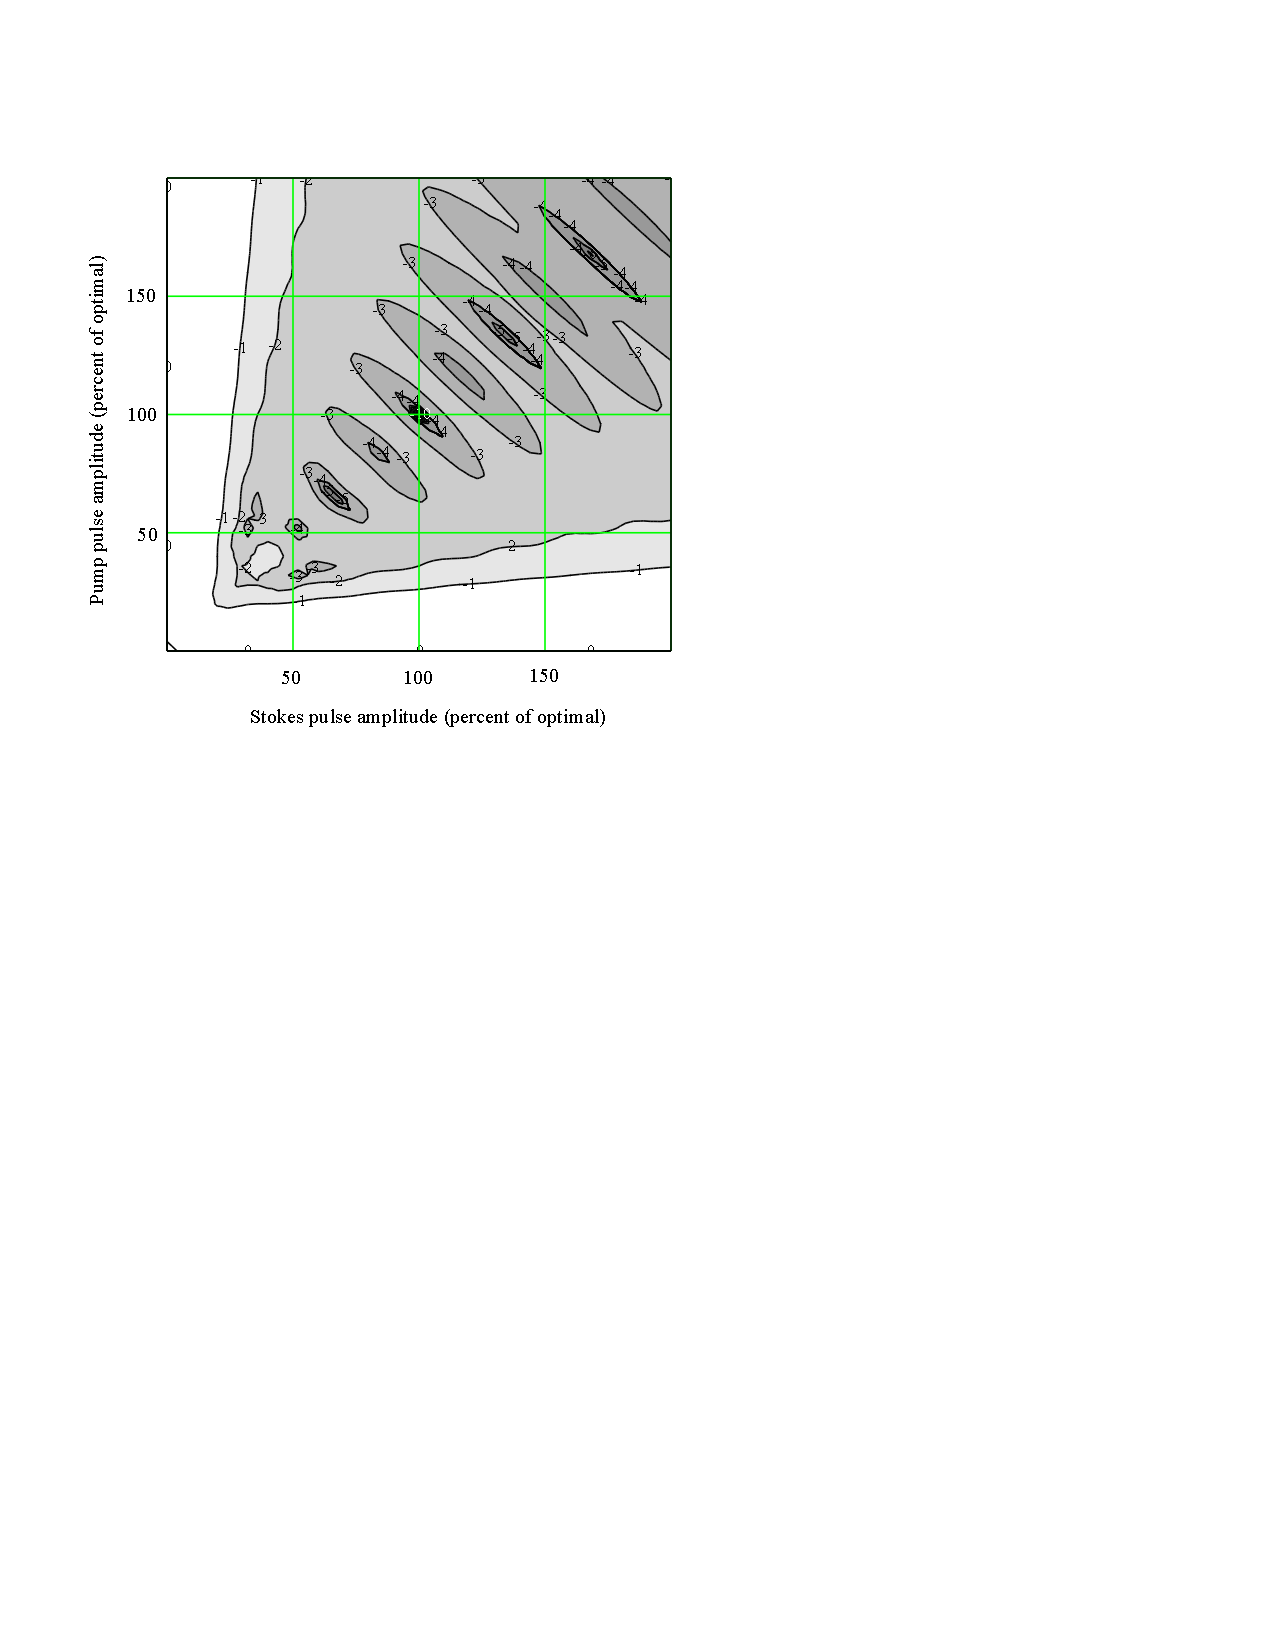
\includegraphics[bb=-15 450 489 700]
{amp_surface/amp_surface.pdf}
}
\caption[Residue surface for various pulse intensities]{Residue surface for various pulse intensities.}
\label{amp_surface}
\end{figure}
%----------------------------------------------------------------------------

%----------------------------------------------------------------------------
One important feature of the STIRAP process is the independence of the inversion on pulse height (first discussed in Chapter \ref{computer chapter}). Figure \ref{amp_surface} shows the surface
\begin{equation}
\Phi^{\prime}
=
1 - P_2(t_N)
\label{phi prime}
\end{equation}
with respect to the amplitudes of the two pulses in the two color solution (STIRAP) shown in Figure \ref{solution 2 pulses}. $\Phi^{\prime}$ is defined in a manner similar to Equation \ref{residue cost} - in fact, the surface in Figure \ref{amp_surface} is similar to, but not the same as, the surface in Figure \ref{amp amp}. Since $\Phi^{\prime}\sim0$ means the inversion was mostly complete, we see that for a majority of the transitions shown in Figure \ref{amp_surface} the inversion was complete to better than 1 part per thousand. Figure \ref{scale_two-color} shows $\Phi^{\prime}$ for the case of simultaneous scaling of the pulses. Compare this to Figure \ref{scale_three-color} where the three color STIRAP is analyzed in a similar way, and we see that the three color STIRAP does not exhibit the same ``robustness'' to pulse amplitude scaling.
%----------------------------------------------------------------------------
%----------------------------------------------------------------------------
%bb defines the bounding box for the pdf
%viewport defines the area of the pdf used
%in sidewaysfigure the last entry in bb moves the caption toward/away the pic
%in sidewaysfigure the second entry in bb moves the pic toward/away the caption
%----------------------------------------------------------------------------
\begin{figure}
\scalebox{0.8}[0.8]{
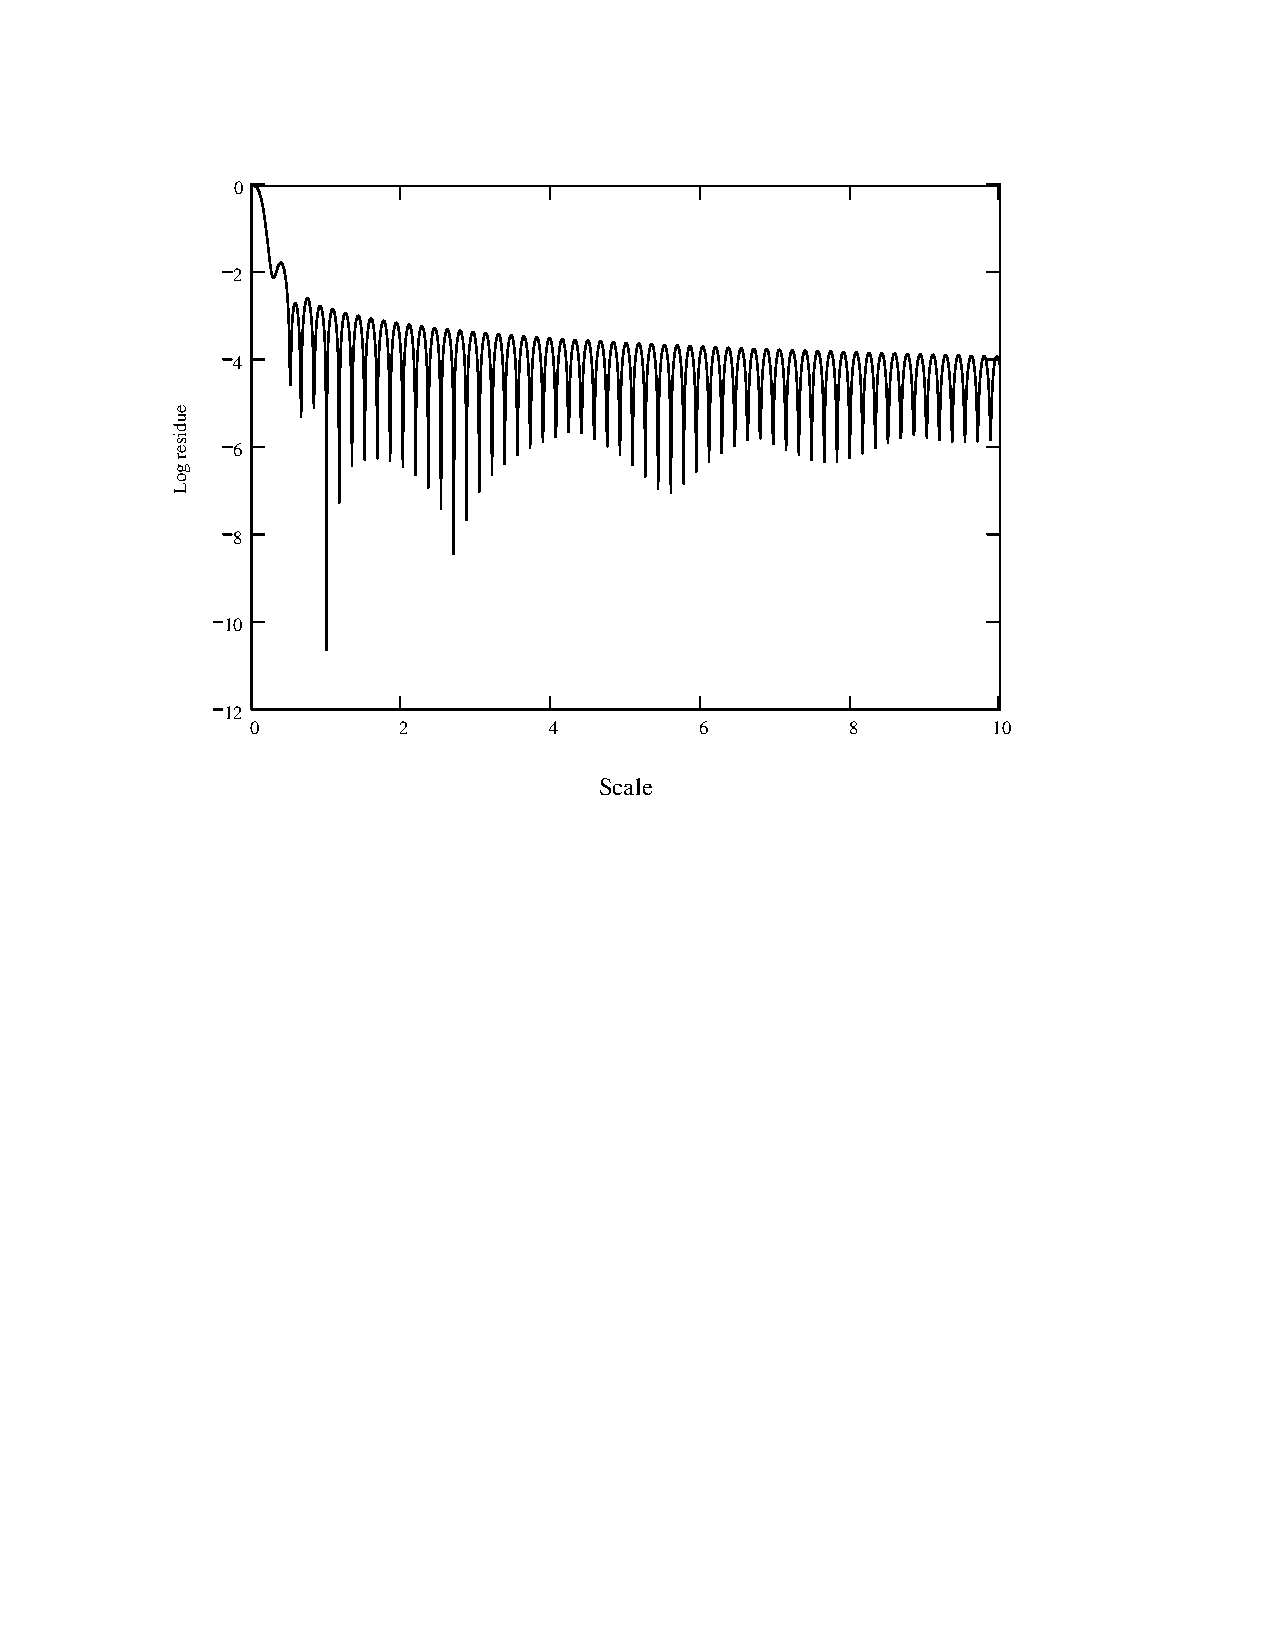
\includegraphics[bb=30 415 489 715]
{scale_two-color/scale_two-color.pdf}
}
\caption[Amplitude ``robustness'' of the two color STIRAP]{Amplitude ``robustness'' of the two color STIRAP. The optimal solution in Figure \ref{solution 2 pulses} is allowed to vary in pulse height by the ``scale'' factor (both pulses are scaled simultaneously) and the resulting residue, as defined by Equation \ref{phi prime} is plotted as a function of the scale. The narrow downward ``spikes'' are real; however, their depth may not be acurately displayed here due to ``aliasing'' effects between the regular spacing of computer generated points and the sharp spikes. In short, the residue is around $10^{-3}$ for most of the range of the ``scale'' factor, except for numerous ``pits'' where the residue drops to $10^{-6}$ or less.}
\label{scale_two-color}
\end{figure}
%----------------------------------------------------------------------------

%----------------------------------------------------------------------------
%----------------------------------------------------------------------------
%----------------------------------------------------------------------------
%bb defines the bounding box for the pdf
%viewport defines the area of the pdf used
%in sidewaysfigure the last entry in bb moves the caption toward/away the pic
%in sidewaysfigure the second entry in bb moves the pic toward/away the caption
%----------------------------------------------------------------------------
\begin{figure}
\scalebox{0.8}[0.8]{
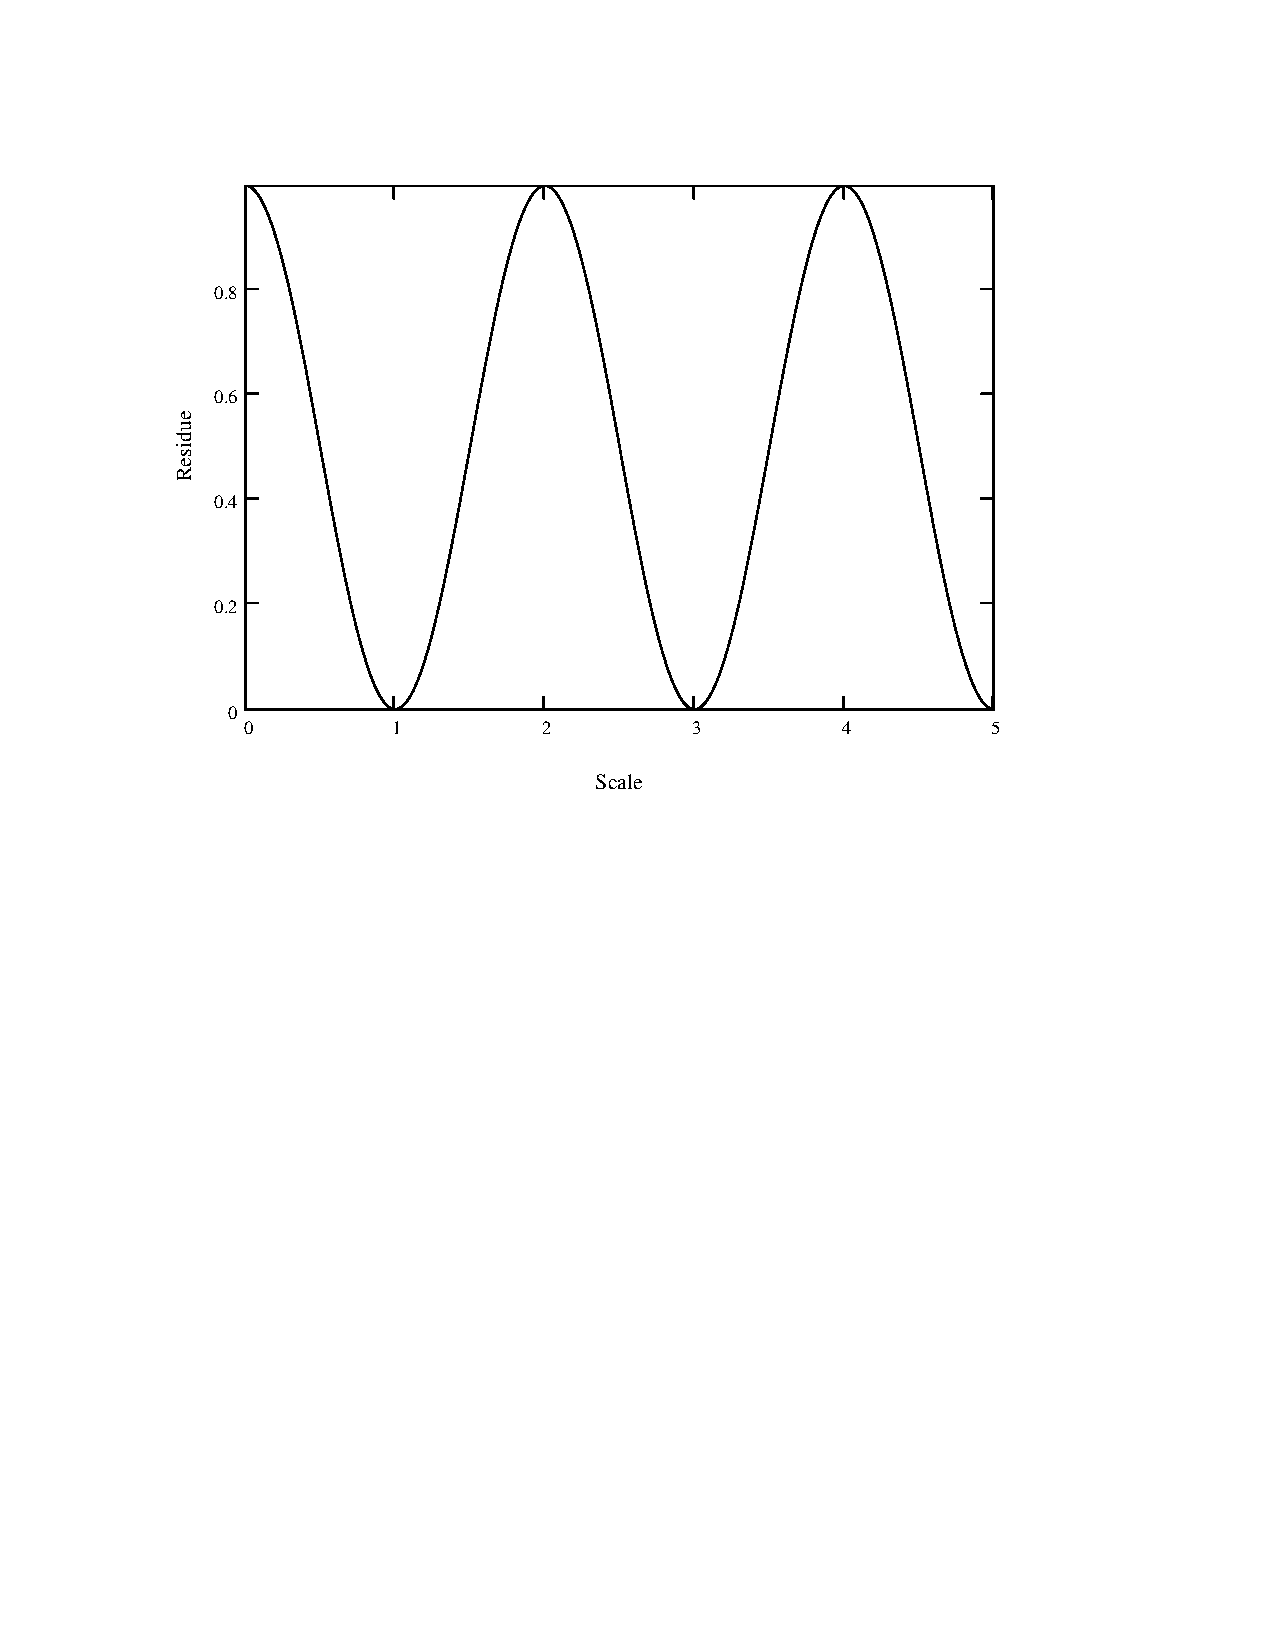
\includegraphics[bb=30 415 489 715]
{scale_three-color/scale_three-color.pdf}
}
\caption[Amplitude ``non-robustness'' of the three color STIRAP]{Amplitude ``non-robustness'' of the three color STIRAP. The optimal solution in Figure \ref{solution three pulses} is allowed to vary in pulse height by the ``scale'' factor (all three pulses are scaled simultaneously) and the resulting residue, as defined by Equation \ref{phi prime} is plotted as a function of the scale.}
\label{scale_three-color}
\end{figure}
%----------------------------------------------------------------------------

%----------------------------------------------------------------------------

%----------------------------------------------------------------------------
%----------------------------------------------------------------------------

%----------------------------------------------------------------------------
%bb defines the bounding box for the pdf
%viewport defines the area of the pdf used
%in sidewaysfigure the last entry in bb moves the caption toward/away the pic
%in sidewaysfigure the second entry in bb moves the pic toward/away the caption
%----------------------------------------------------------------------------
\begin{figure}
\scalebox{0.8}[0.8]{
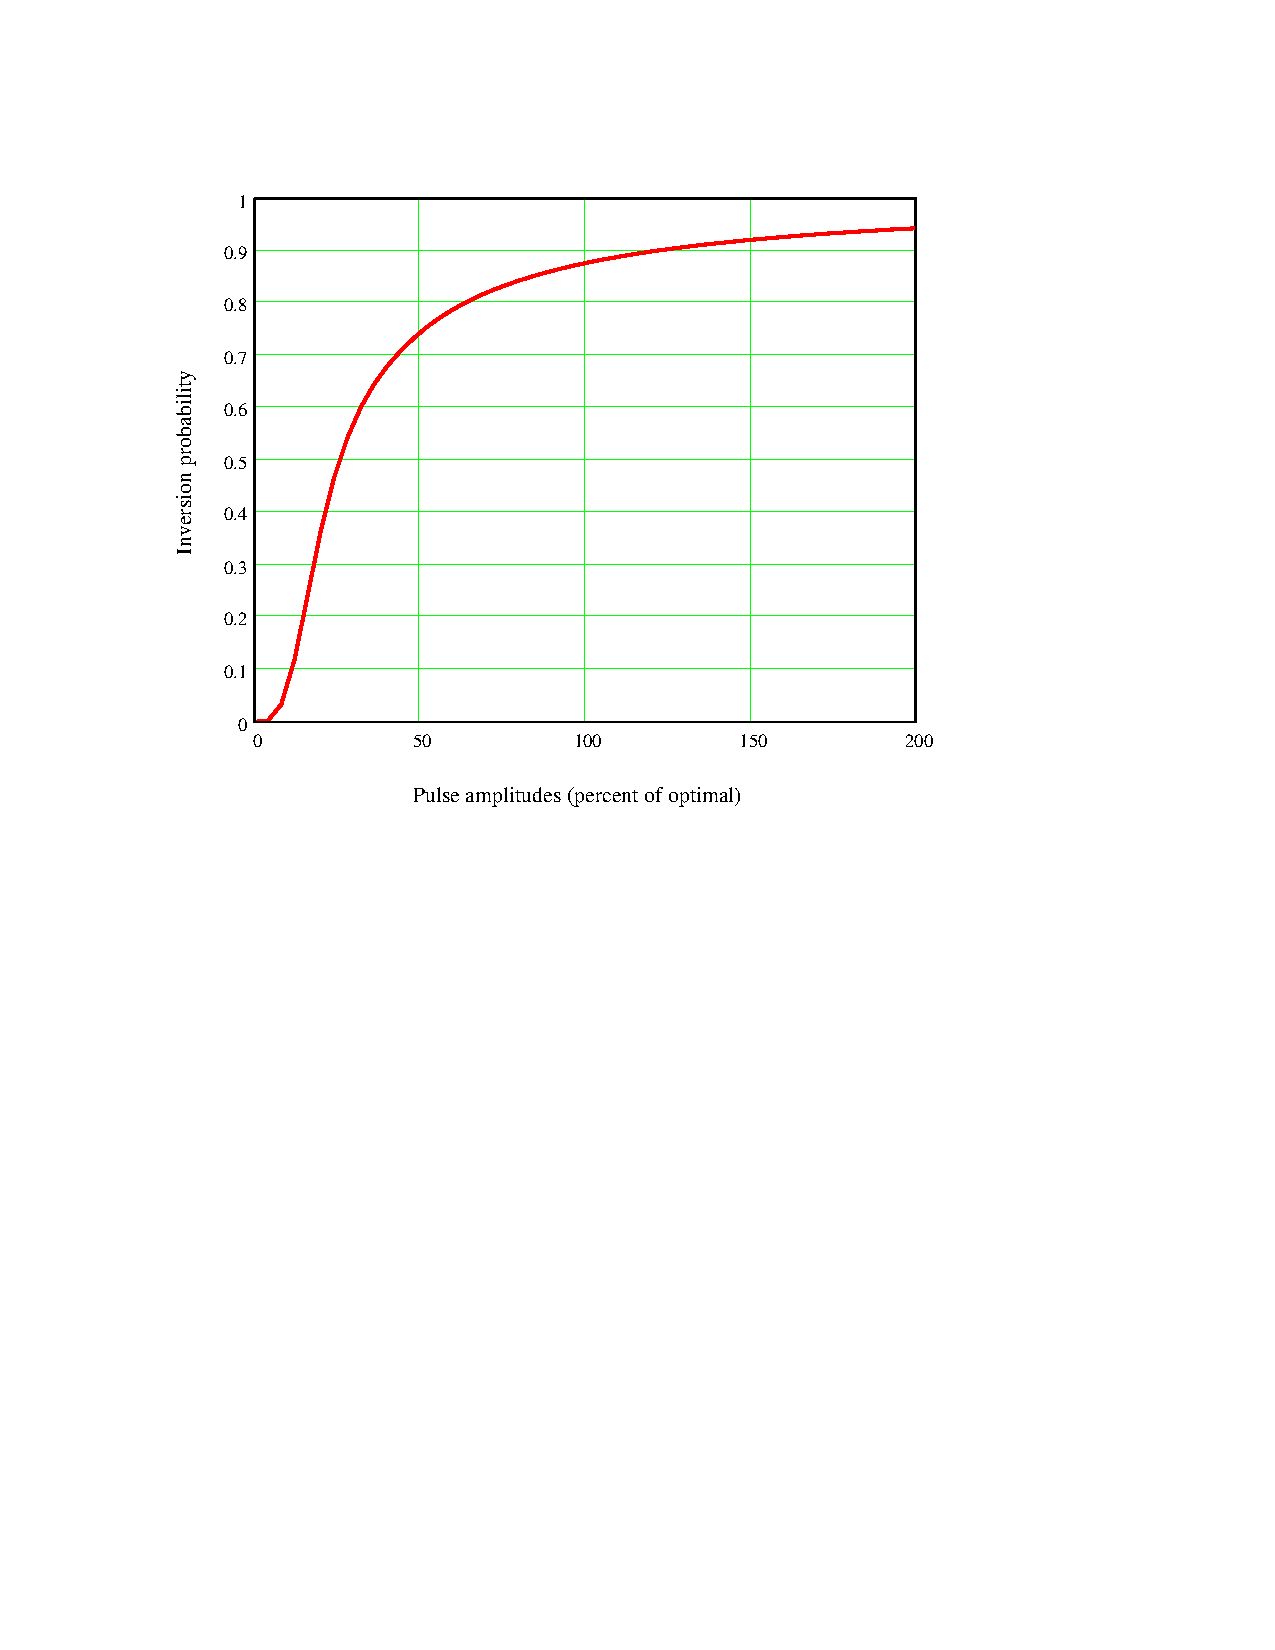
\includegraphics[bb=10 415 489 700]
{polarization/polarization.pdf}
}
\caption[STIRAP inversion of a randomly oriented ensemble]{STIRAP inversion of a randomly oriented ensemble. Compare this with the dynamics shown in Figure \ref{dynamics} and we see that the STIRAP process approaches a coherent 100\% inversion in the semi--classical analysis of a randomly orientated ensemble while the standard single color method of inverting the ensemble tends toward an incoherent 50\% inversion with oscillations.}
\label{polarization}
\end{figure}
%----------------------------------------------------------------------------

%----------------------------------------------------------------------------
%----------------------------------------------------------------------------
%----------------------------------------------------------------------------
%bb defines the bounding box for the pdf
%viewport defines the area of the pdf used
%in sidewaysfigure the last entry in bb moves the caption toward/away the pic
%in sidewaysfigure the second entry in bb moves the pic toward/away the caption
%----------------------------------------------------------------------------
\begin{figure}
\scalebox{0.8}[0.8]{
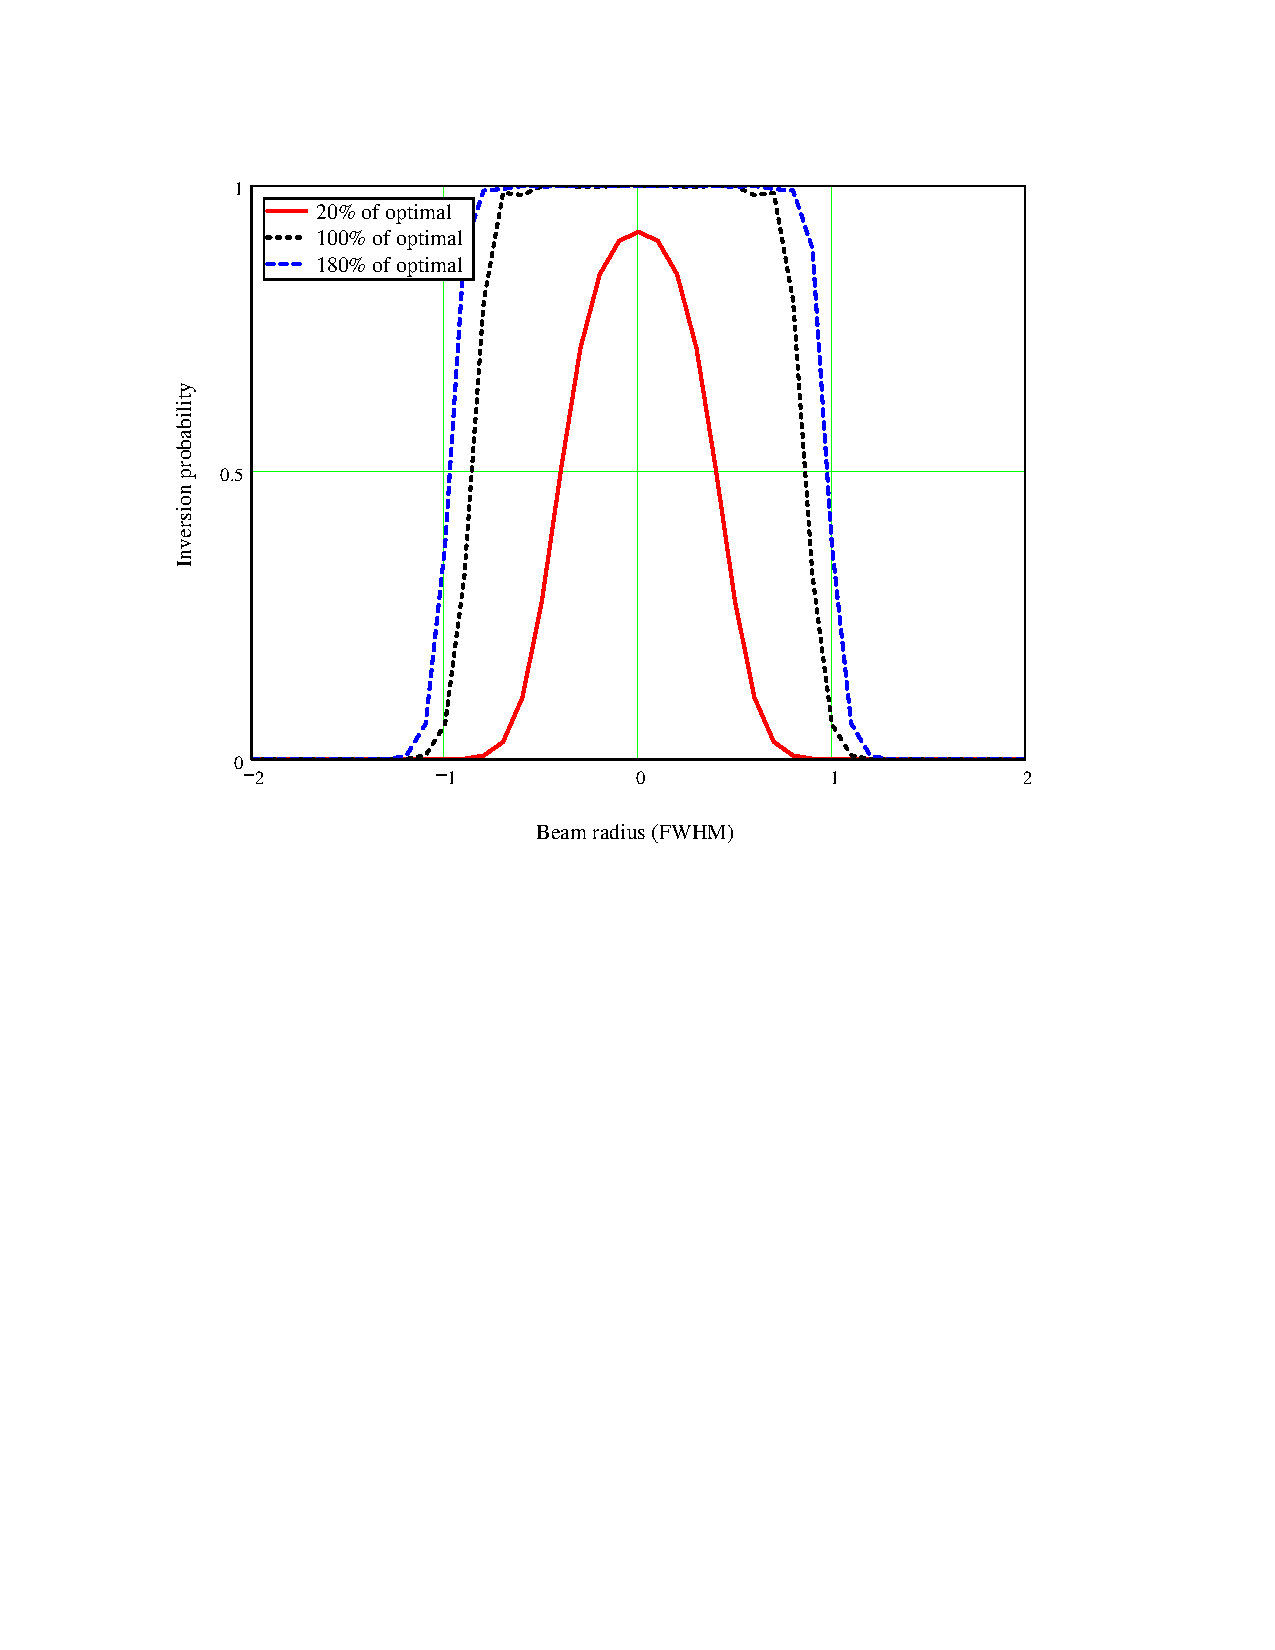
\includegraphics[bb=25 400 489 700]
{gaussian/gaussian.pdf}
}
\caption{Inversion probability across a Gaussian beam profile}
\label{gaussian}
\end{figure}
%----------------------------------------------------------------------------

%----------------------------------------------------------------------------
The STIRAP process also turns out to be beneficial when one considers the spatial distribution of the inverted molecules an a Gaussian beam. The pulse amplitudes are allowed to vary as a pair (the pulses remain of equal height) and the population inversion is calculated across the cross section of Gaussian beam. We see in Figure \ref{gaussian} we see that near top hat cross section are possible.
%----------------------------------------------------------------------------
%----------------------------------------------------------------------------
%----------------------------------------------------------------------------

%----------------------------------------------------------------------------
\subsection{The STIRAP detuning ridge}
%----------------------------------------------------------------------------
\label{STIRAP ridge section}
%----------------------------------------------------------------------------
%----------------------------------------------------------------------------
%----------------------------------------------------------------------------
\begin{figure}
\begin{center}
\leavevmode
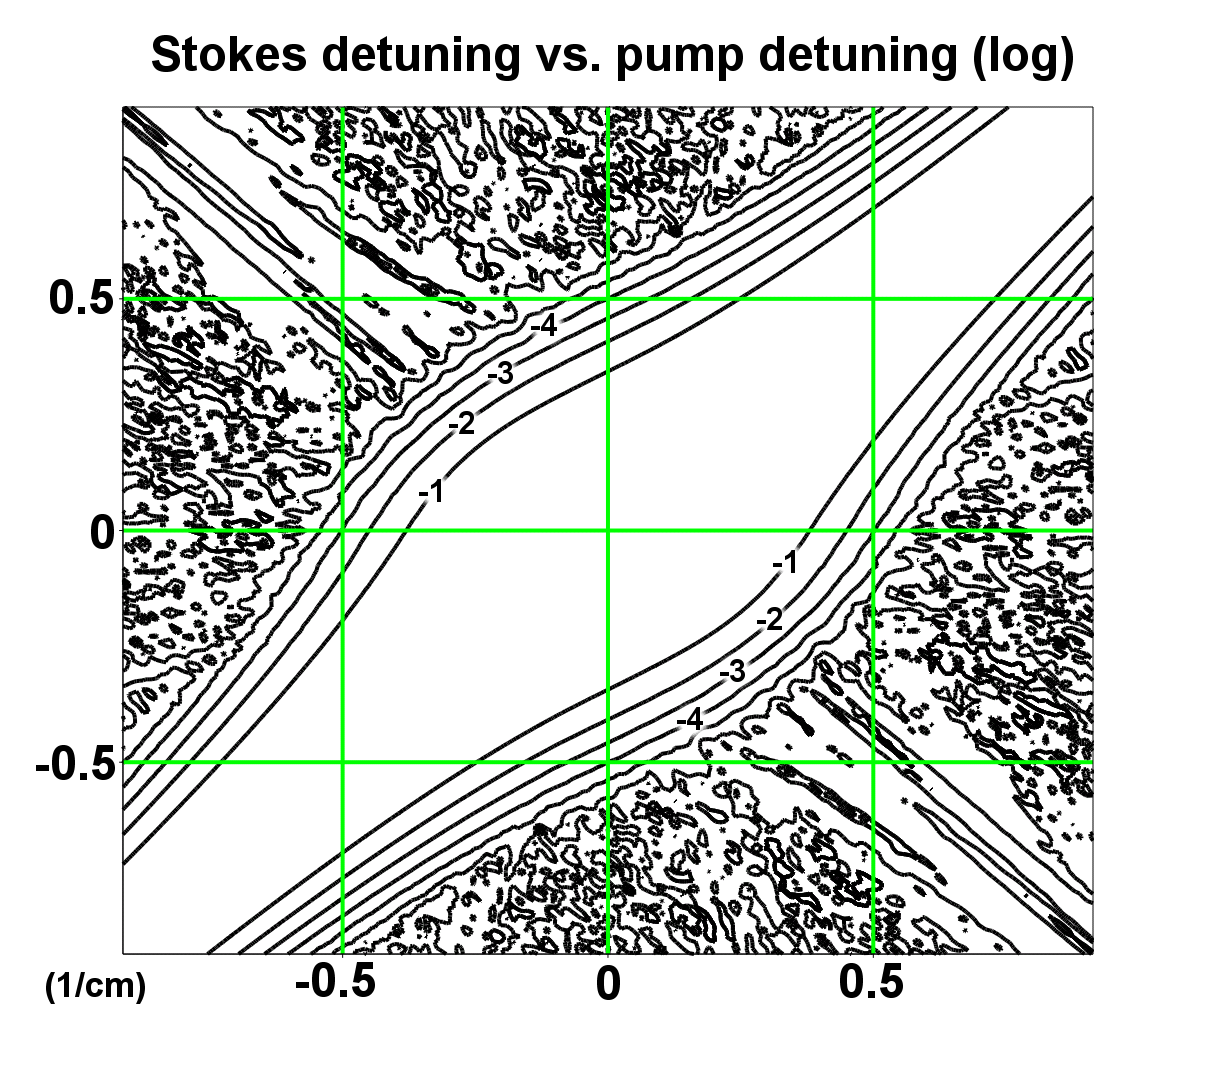
\includegraphics[width=4in]
{ridge/ridge.png}\\
\end{center}
\caption[STIRAP detuning ridge]{STIRAP detuning ridge - The log of the inversion probability is plotted here. See Figure \ref{sp_detuning} for the definition of the Stokes pulse and the pump pulse.}
\label{ridge}
\end{figure} 
%----------------------------------------------------------------------------

%----------------------------------------------------------------------------
%bb defines the bounding box for the pdf
%viewport defines the area of the pdf used
%in sidewaysfigure the last entry in bb moves the caption toward/away the pic
%in sidewaysfigure the second entry in bb moves the pic toward/away the caption
%----------------------------------------------------------------------------
\begin{figure}
\scalebox{0.8}[0.8]{
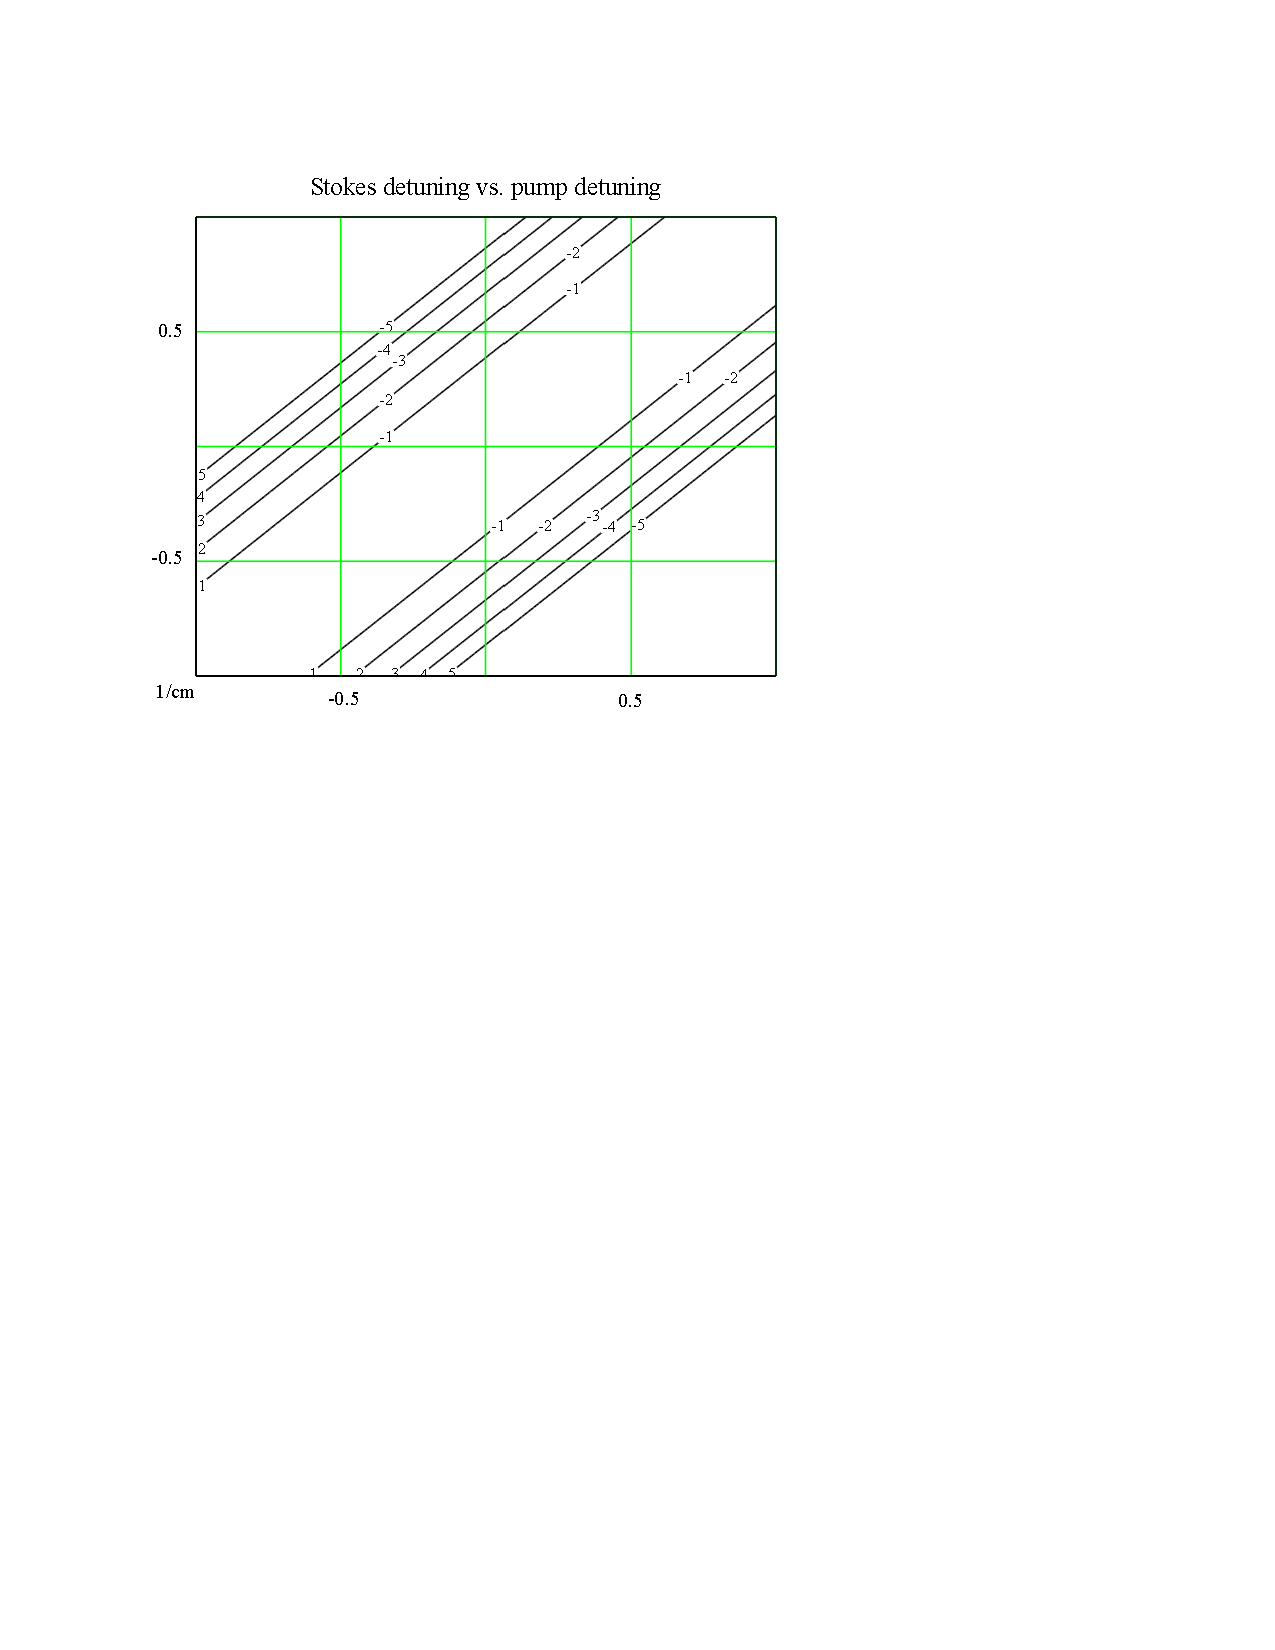
\includegraphics[bb=-30 430 489 700]
{ridge_fit/ridge_fit.pdf}
}
\caption[STIRAP detuning ridge fit]{STIRAP detuning ridge fit - The log of the inversion probability is plotted here.}
\label{ridge_fit}
\end{figure}
%----------------------------------------------------------------------------

%----------------------------------------------------------------------------
The STIRAP process has a unique ``detuning'' feature very different from the corresponding feature for two sequential $\pi$--pulses. The single $\pi$--pulse detuning curve is a sinusoid modulated by a relatively wide Lorentzian (see Section \ref{doppler section}) . The FWHM of this Lorentzian is half the Rabi frequency or, in order to beat the relaxation effects in atmospheric conditions, about one half GHz. This is on the order of the Doppler broadening, so for this discussion, the overall Lorentzian width of a single $\pi$--pulse is near 0.03 inverse cm. To obtain the two $\pi$--pulse detuning line shape we plot the surface formed by the inversion probability as a function of the first pulse (Stokes) detuning and the second pulse (pump) detuning and we get a Lorentzian ``mountain'' with a rough FWHM of 0.03 inverse cm (see Figure \ref{sp_detuning} for the definition of the Stokes pulse and the pump pulse).
%----------------------------------------------------------------------------
%----------------------------------------------------------------------------
%bb defines the bounding box for the pdf
%viewport defines the area of the pdf used
%in sidewaysfigure the last entry in bb moves the caption toward/away the pic
%in sidewaysfigure the second entry in bb moves the pic toward/away the caption
%----------------------------------------------------------------------------
\begin{figure}
\scalebox{0.6}[0.6]{
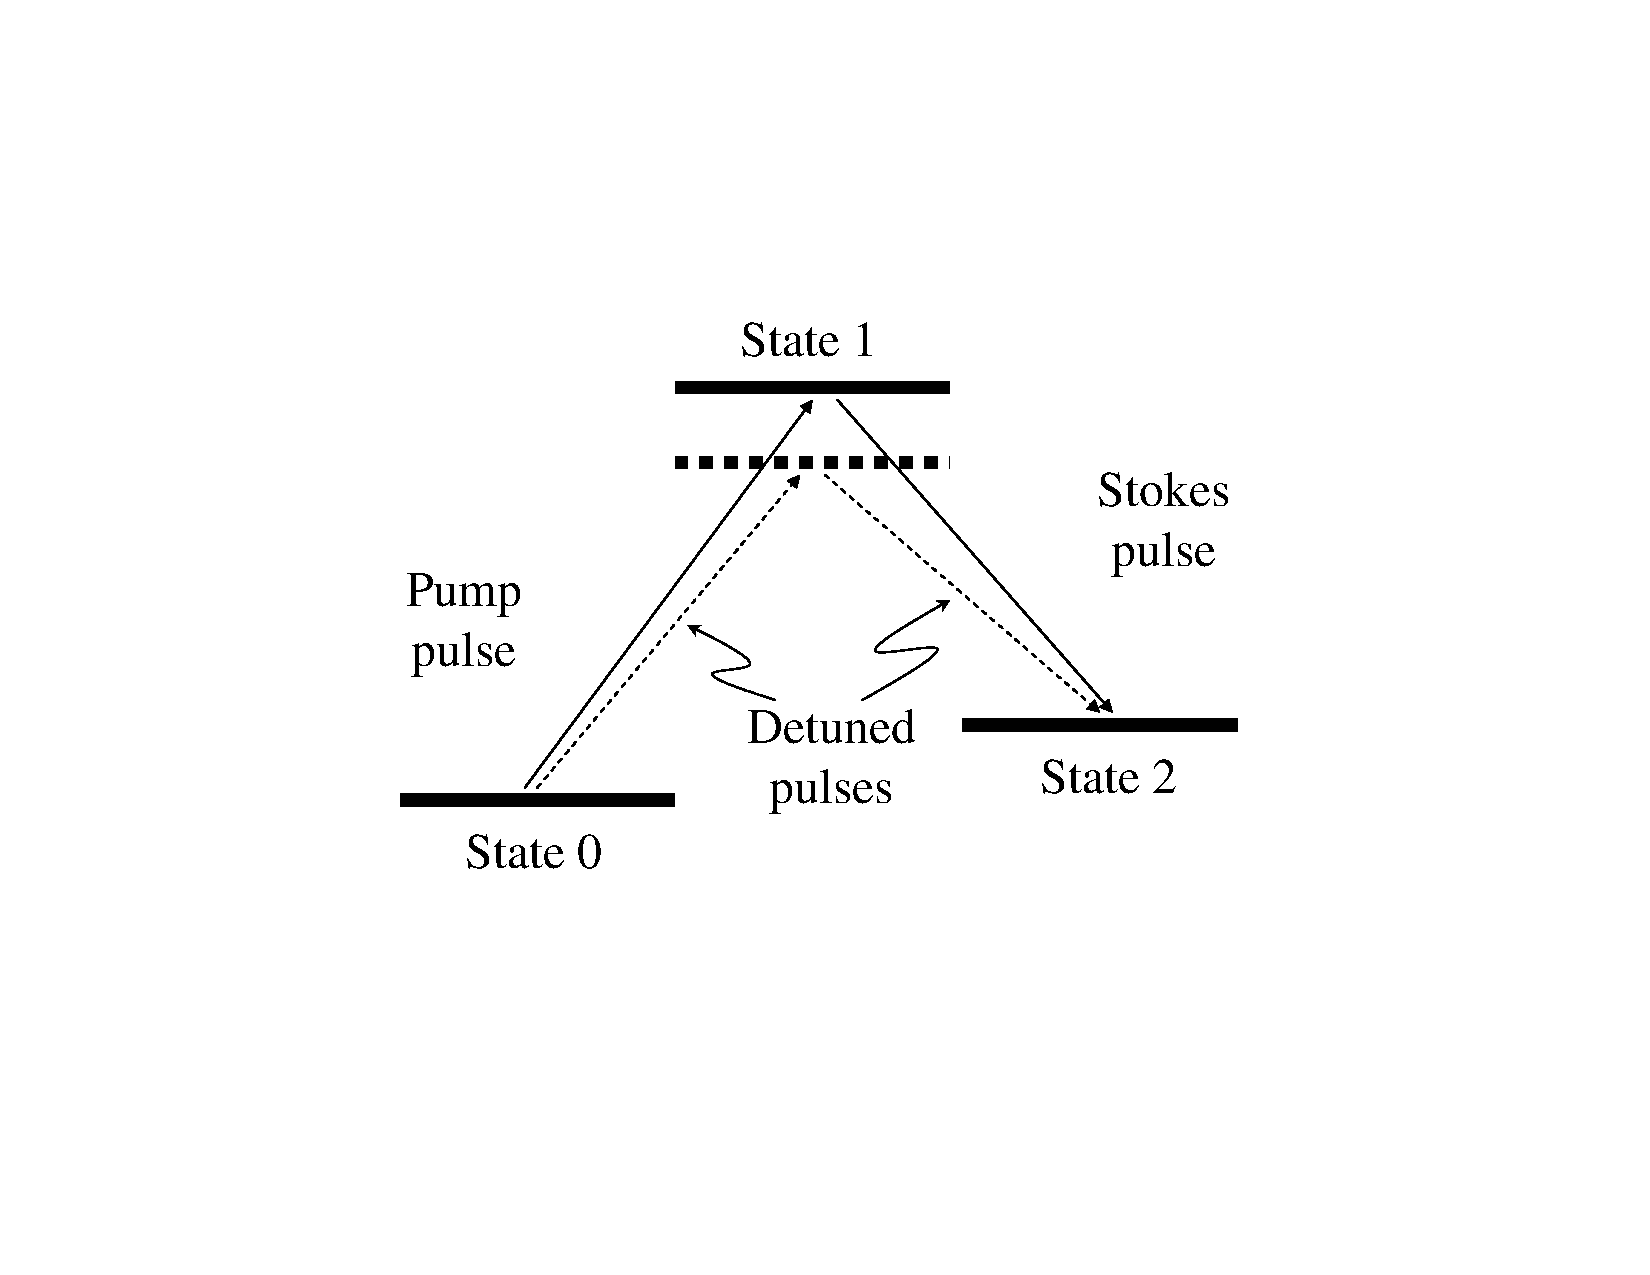
\includegraphics[bb=35 180 489 450]
{sp_detuning/sp_detuning.pdf}
}
\caption[Stokes and pump pulses in a $\Lambda$ system]{Stokes and pump pulses in a $\Lambda$ system. Here we show the pump pulse (connecting states $\ket{0}$ and $\ket{1})$ and the stokes pulse (connecting states $\ket{1}$ and $\ket{2})$. In Figure \ref{amp_surface} we show the effect of amplitude variations on the residue. Also shown here are two \emph{equally} detuned pulses. The figure suggests that significant population will still transfer, but only when the detunings are nearly equal. See Figure \ref{ridge} for an actual calculation.}
\label{sp_detuning}
\end{figure}
%----------------------------------------------------------------------------

%----------------------------------------------------------------------------

To obtain a similar detuning feature for the STIRAP process we start with Equation \ref{dim eom}, obtain equations similar to Equations \ref{doppler eom}, apply the STIRAP pulse sequence, and numerically calculate the inversion probability for various detunings. It is found that (see Figure \ref{ridge}) the detuning feature is a ridge with a long extent along the ridge (roughly fits a Lorentzian with a FWHM of 21.2 inverse cm) and a sharp fall-off along the anti-ridge (roughly fits a Gaussian with a FWHM of 0.424 inverse cm).
%----------------------------------------------------------------------------
%----------------------------------------------------------------------------
%bb defines the bounding box for the pdf
%viewport defines the area of the pdf used
%in sidewaysfigure the last entry in bb moves the caption toward/away the pic
%in sidewaysfigure the second entry in bb moves the pic toward/away the caption
%----------------------------------------------------------------------------
\begin{figure}
\scalebox{0.8}[0.8]{
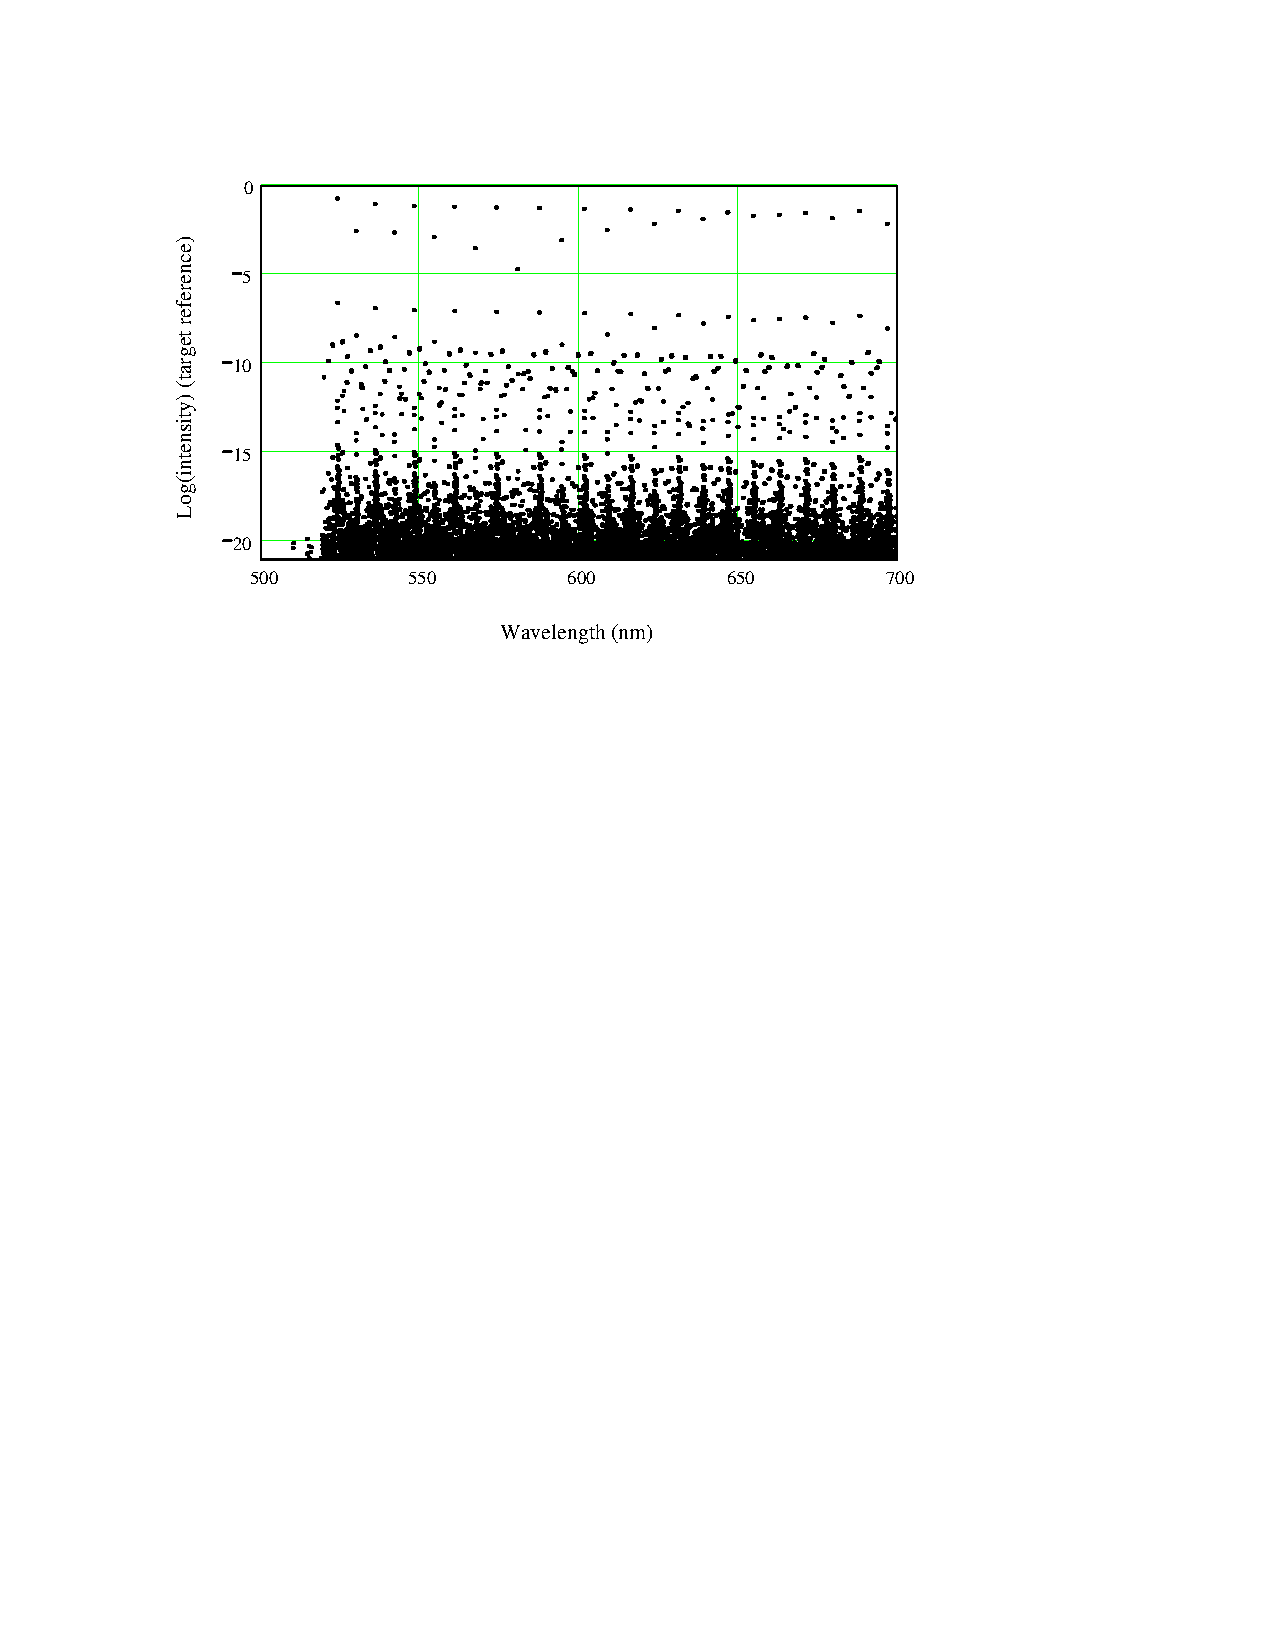
\includegraphics[bb=0 480 489 752]
{PI_79/PI_79.pdf}
}
\caption[Simulated three $\pi$--pulse pathway LIF line strengths (target)]{Simulated three $\pi$--pulse pathway LIF line strengths (target)}
\label{PI_79}
\end{figure}
%----------------------------------------------------------------------------

%----------------------------------------------------------------------------
%bb defines the bounding box for the pdf
%viewport defines the area of the pdf used
%in sidewaysfigure the last entry in bb moves the caption toward/away the pic
%in sidewaysfigure the second entry in bb moves the pic toward/away the caption
%----------------------------------------------------------------------------
\begin{figure}
\scalebox{0.8}[0.8]{
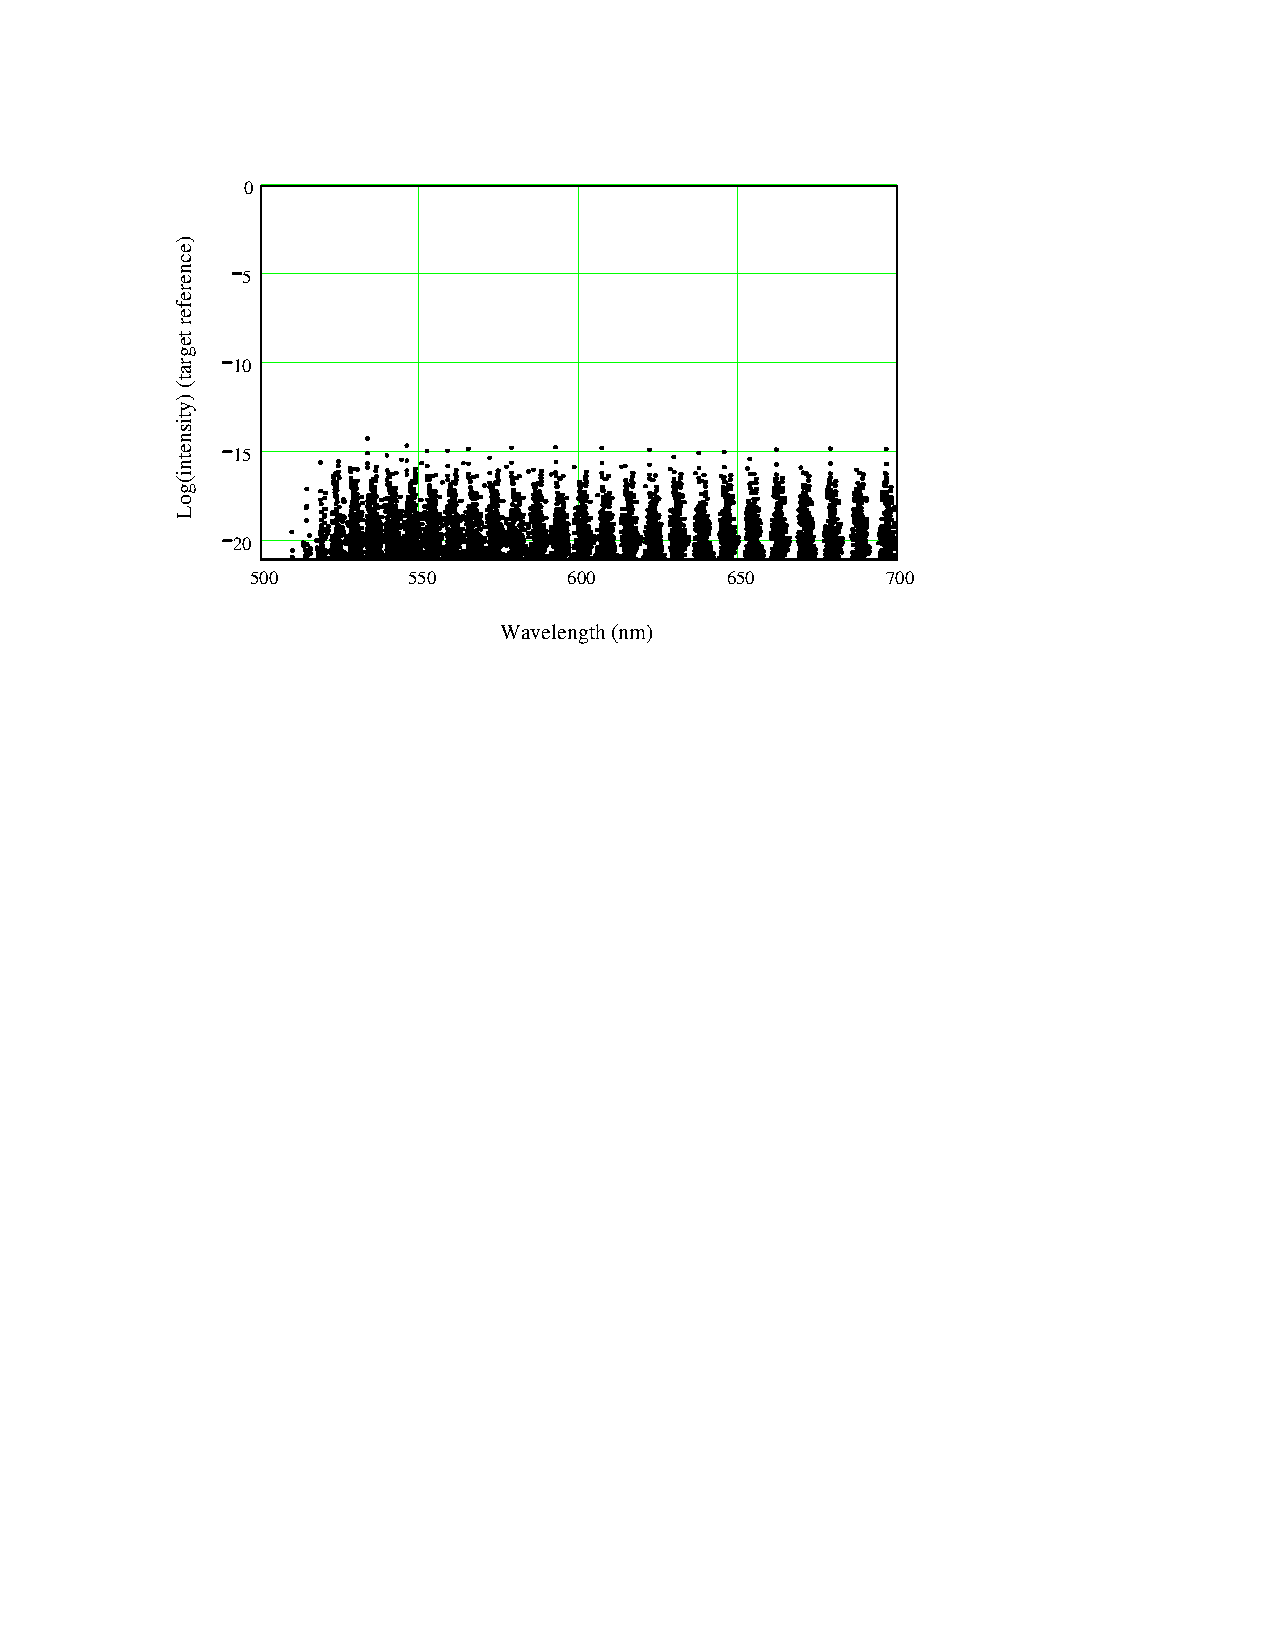
\includegraphics[bb=0 480 489 752]
{PI_77/PI_77.pdf}
}
\caption[Simulated three $\pi$--pulse pathway LIF line strengths (non-target)]{Simulated three $\pi$--pulse pathway LIF line strengths (non-target)}
\label{PI_77}
\end{figure}
%----------------------------------------------------------------------------

%----------------------------------------------------------------------------

To model the effects of this detuning feature of the STIRAP process on the fluorescence spectrum we fit the ridge to an analytic function and use this fit in the computer model described in Section \ref{approx section}. The Lorentzian in Equation \ref{main approx} is replaced with the ridge fit (see Figure \ref{ridge_fit}) and a resulting fluorescence spectrum is calculated.

To compare the STIRAP + $\pi$--pulse (scheme 1) to the three $\pi$--pulse (scheme 2) scheme, we generate plots similar to Figure \ref{target_3}; however, instead of attaching Lorentzian line shapes to each LIF transition we simply plot each transition. See Figure \ref{STIRAP_79} for a plot of the LIF transition supported by scheme 1 for the target molecule, Figure \ref{STIRAP_77} for scheme 1 on the non-target molecule. Compare these plots with Figures \ref{PI_79} and \ref{PI_77} and one sees that scheme 1 ``pulls'' more transitions through the three color pathway than scheme 2. This is one drawback of the robustness of the STIRAP process; however, it does not adversely affect the selectivity of the process since the Lorentzian tail of the fluorescence still dominates (see Figure \ref{target_3} and \ref{non-target_1}).
%----------------------------------------------------------------------------
%----------------------------------------------------------------------------
%bb defines the bounding box for the pdf
%viewport defines the area of the pdf used
%in sidewaysfigure the last entry in bb moves the caption toward/away the pic
%in sidewaysfigure the second entry in bb moves the pic toward/away the caption
%----------------------------------------------------------------------------
\begin{figure}
\scalebox{0.8}[0.8]{
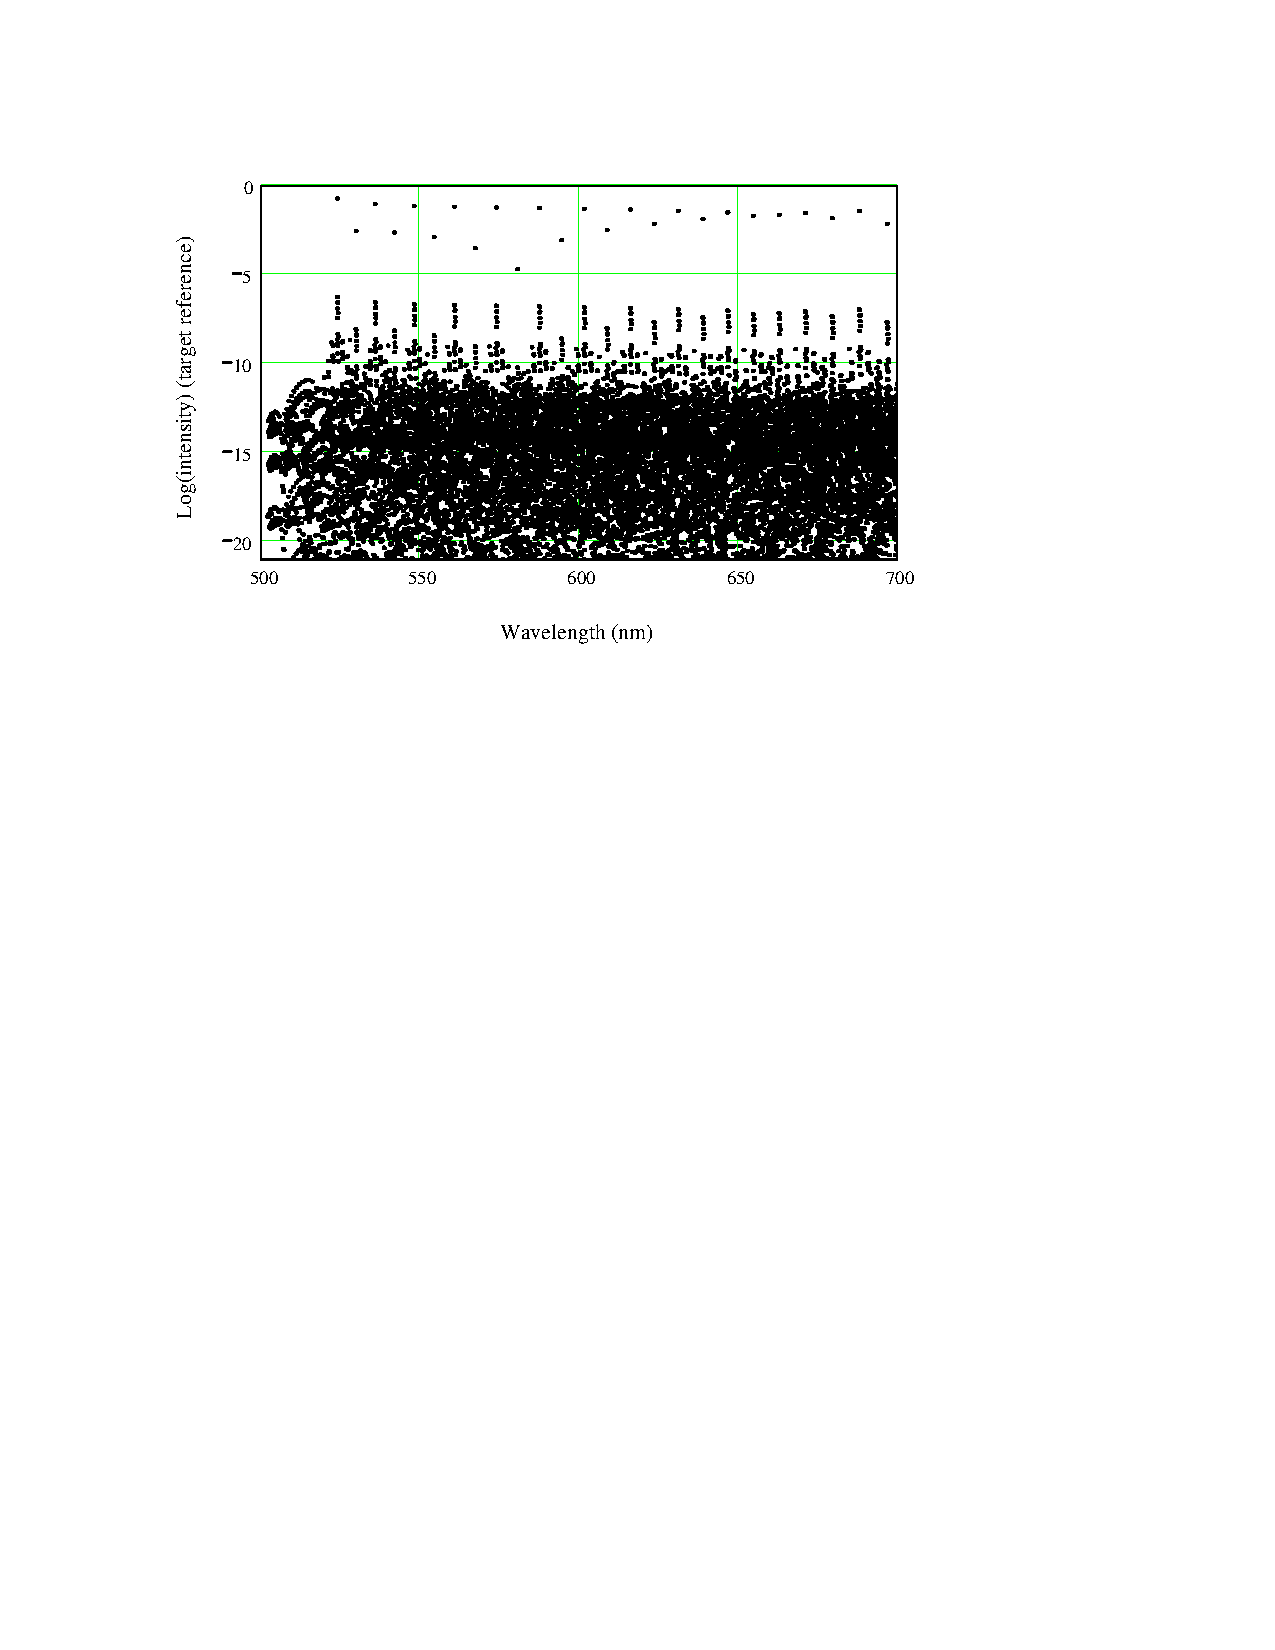
\includegraphics[bb=0 480 489 752]
{STIRAP_79/STIRAP_79.pdf}
}
\caption[Simulated STIRAP + $\pi$--pulse pathway LIF line strengths (target)]{Simulated STIRAP + $\pi$--pulse pathway LIF line strengths (target)}
\label{STIRAP_79}
\end{figure}
%----------------------------------------------------------------------------

%----------------------------------------------------------------------------
%bb defines the bounding box for the pdf
%viewport defines the area of the pdf used
%in sidewaysfigure the last entry in bb moves the caption toward/away the pic
%in sidewaysfigure the second entry in bb moves the pic toward/away the caption
%----------------------------------------------------------------------------
\begin{figure}
\scalebox{0.8}[0.8]{
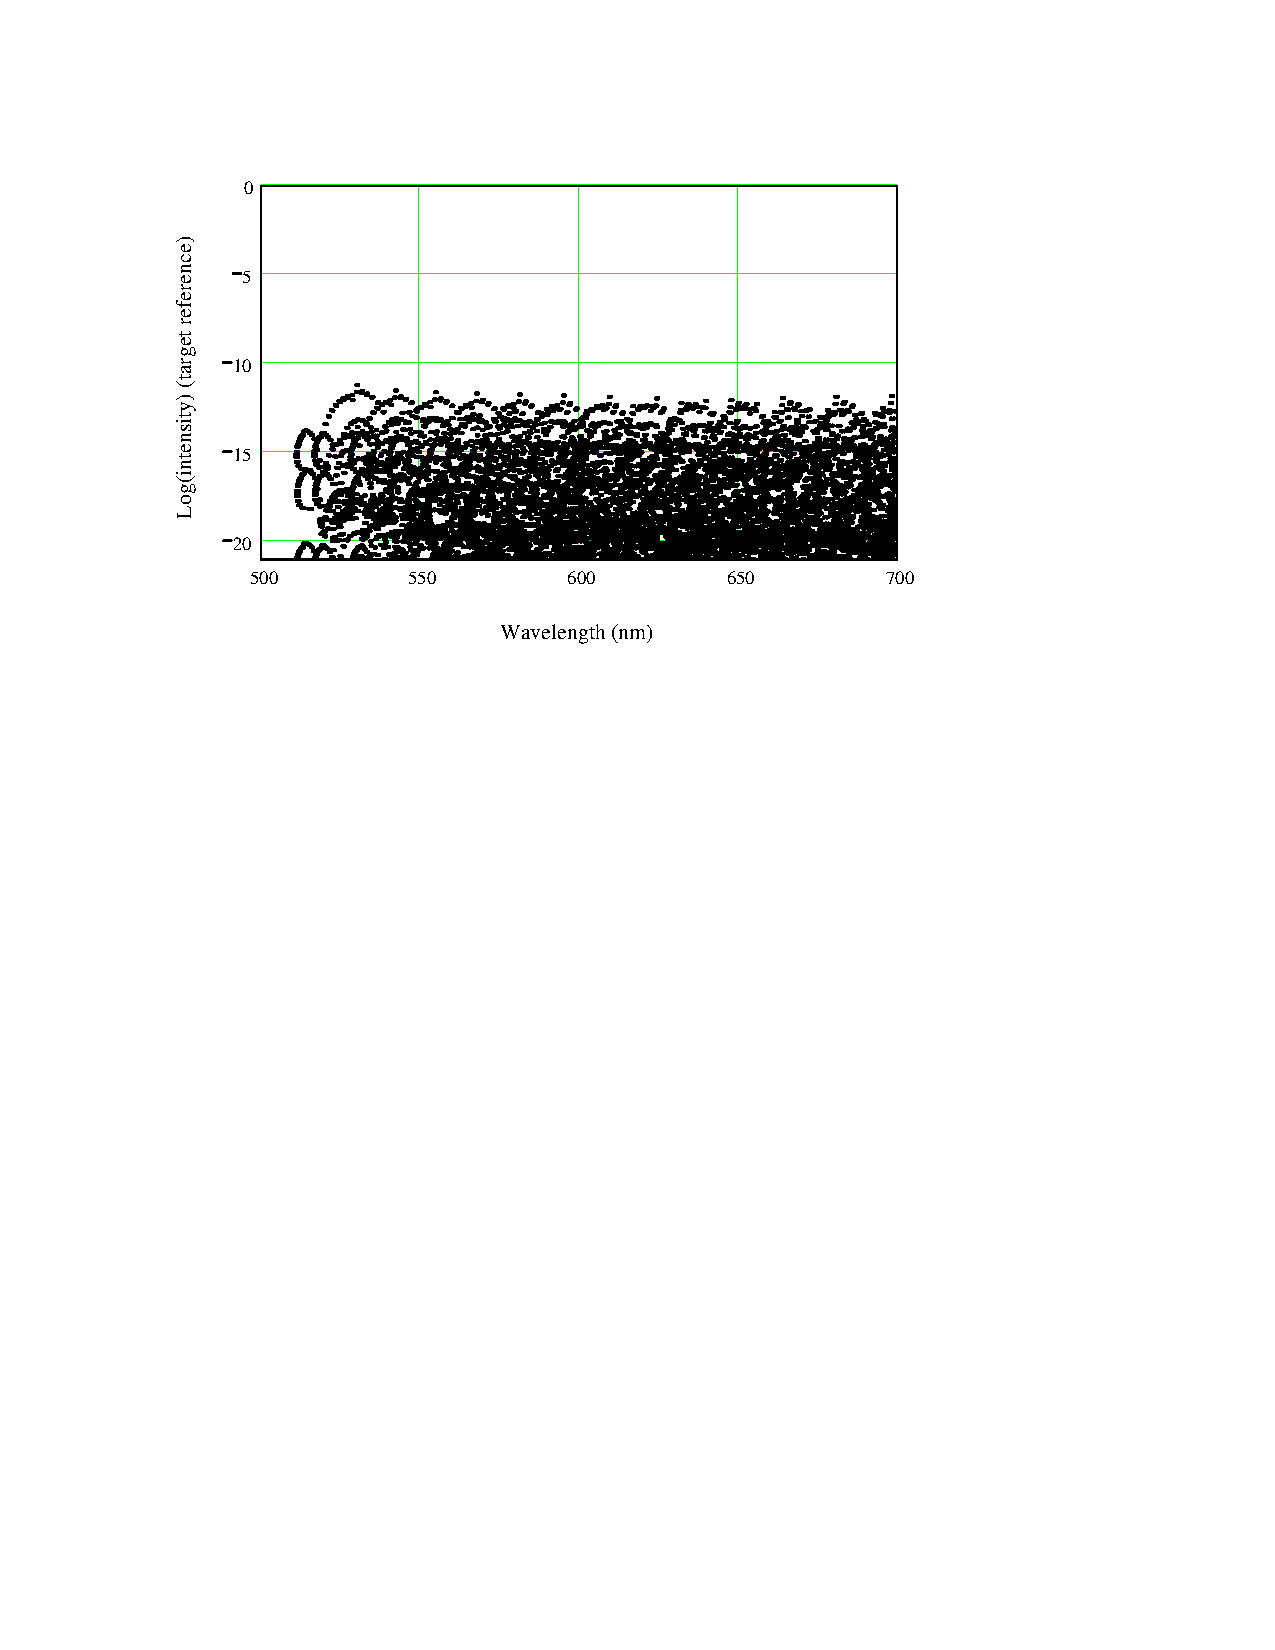
\includegraphics[bb=0 480 489 752]
{STIRAP_77/STIRAP_77.pdf}
}
\caption[Simulated STIRAP + $\pi$--pulse pathway LIF line strengths (non-target)]{Simulated STIRAP + $\pi$--pulse pathway LIF line strengths (non-target)}
\label{STIRAP_77}
\end{figure}
%----------------------------------------------------------------------------

%----------------------------------------------------------------------------
%----------------------------------------------------------------------------

%----------------------------------------------------------------------------
%----------------------------------------------------------------------------
\section{Conclusion}
%----------------------------------------------------------------------------
%------------------------------Broad objectives------------------------------
%----------------------------------------------------------------------------
This chapter chronicles the stages of laboratory development undergone over the past few years. The main measurements at each stage were used as a guide to develop the equipment and techniques required for demonstration of molecular control in LIDAR systems.
%----------------------------------------------------------------------------
%----------------------------------So what?----------------------------------
%----------------------------------------------------------------------------

As each stage was completed various components of the apparatus were either designed and assembled or evolved to the next generation. After the installation of the PMT at its output the monochromator served each experiment well until the recent aromatic compound measurements. The Hg pulser and Pockles cell system went through various stages of development starting with the initial tests of the Hg pulser on LED's to the integration of the system with the YAG pumped dye laser system during the fluorescence line decay measurements. The software model was tested at each stage from the familiar non-resonant HeNe LIF to pulsed resonant dye LIF. The data acquisition system was built for the first dye laser experiments and has remained relatively unchanged since then. Recently, a calibration issue with the monochromator self scan feature has prompted the need of a second generation of the data acquisition software.
%----------------------------------------------------------------------------
%---------------------------------Synthesize---------------------------------
%----------------------------------------------------------------------------
%----------------------------------------------------------------------------
%----------------------------------------------------------------------------
%----------------------------------------------------------------------------

%----------------------------------------------------------------------------
%----------------------------------------------------------------------------
